\documentclass[11pt]{article}


%\input{meta/packages}
%
\usepackage{cite}
\usepackage[T1]{fontenc}
\usepackage{times}
\usepackage{url}
\usepackage{amsmath}
\usepackage{fancyhdr}
\usepackage{fancyvrb}
\usepackage{fancybox}
\usepackage{color}
\usepackage{colortbl}
\usepackage[table]{xcolor}
%\usepackage{tex-helpers/mathpartir}
\usepackage{amssymb}
\usepackage{xspace}
\usepackage{comment}
\usepackage{graphicx}
\graphicspath{{figures/}}
\usepackage{epsfig}
\usepackage{wrapfig}
\usepackage{multirow}
\usepackage{subfig}

% Added listing for code listings
\usepackage{listings}
\usepackage{relsize}
\usepackage{setspace}
\usepackage{sidecap}
\usepackage{algorithm}
\usepackage{algorithmic}

\textwidth=16.5cm 
\textheight=22.5cm 
\textwidth=16.5cm 
\textheight=55.5pc
\topmargin=-0.5cm 
\headsep=0cm 
\headheight=0cm 
\oddsidemargin=0cm
\evensidemargin=0cm 
\marginparwidth=0cm
\parskip=0cm
\itemsep=0.1pt
\parindent=0.5cm

%Set table separation 
\setlength{\tabcolsep}{1pt}

% Allow figures to take up the entire page
\renewcommand\floatpagefraction{.99}
\renewcommand\topfraction{.99}
\renewcommand\bottomfraction{.90}
\renewcommand\textfraction{.01}   
\setcounter{totalnumber}{50}
\setcounter{topnumber}{50}
\setcounter{bottomnumber}{50}

% formatting for grammars
%\input{tex-helpers/obey}
%\input{tex-helpers/grammar}
%\renewcommand{\nonterm}[1]{\mbox{\textit{#1}}}
\newcommand{\oneormore}[1]{#1\ensuremath{^+}}

\newcommand{\opt}[1]{\textbf{[}#1\textbf{]}}

\newcommand{\mc}[1]{\mbox{\rm \ensuremath{\text{\code{#1}}}}} 
\newcommand{\loc}{\ensuremath{\mathord{\mathit{loc}}}}
\newcommand{\ec}{\ensuremath{\mathop{\mathbb{E}}}}
\newcommand{\hole}{\ensuremath{\mathord{\mathit{-}}}}
\newcommand{\reducesto}{\hookrightarrow}

\newcommand*{\seq}[1]{\ensuremath{\left\langle {#1} \right\rangle}}
\newcommand{\config}{\seq}
\newcommand{\udot}{\mathbin{\sqcup \kern-0.53em \cdot \,}}

% Aux functions
\newcommand{\auxFunc}[1]{\ensuremath{\mathop{\mathit{#1}}}}
\newcommand{\concat}{\auxFunc{concat}}
\newcommand{\reverse}{\auxFunc{reverse}}

% Type checking macros
% change symbol type of : from mathrel 
%\DeclareMathSymbol{:}{\mathbin}{operators}{"3A} 
\newcommand{\OK}{\mbox{OK}}
\newcommand{\OKin}{\mbox{OK in }}
\newcommand{\isType}{\mbox{\textit{isType}}}
\newcommand{\isThunkType}{\mbox{\textit{isThunkType}}}
\newcommand{\isClass}{\mbox{\textit{isClass}}}
\newcommand{\Types}{\mbox{\textit{Types}}}
\newcommand{\Names}{\mbox{\textit{Names}}}
\newcommand{\TypeEnv}{\mbox{\textit{TypeEnv}}}
\newcommand{\VD}{\mbox{\textit{VD}}}
\newcommand{\TypesInOrder}{\mbox{\textit{typesInOrder}}}
\newcommand{\dom}{\mbox{\textit{dom}}}
\newcommand{\rng}{\mbox{\textit{rng}}}
\newcommand{\POWERSET}[1]{\mbox{\textit{PowerSet}}(#1)}
\newcommand{\delete}{\mbox{\textit{delete}}}
\newcommand{\mklist}{\mbox{\textit{mksupers}}}
\newcommand{\uminus}{\mbox{$\cup\!\!\!\!-$}}
\newcommand{\iminus}{\mbox{$\cap\!\!\!\!-$}}
\newcommand{\rname}[1]{$\TirName{(#1)}$} % for inline inferrule names
\newcommand{\STO}{\ensuremath{<:}}  % ``subtype of''
\newcommand{\consistent}{\ensuremath{\approx}}

% Notations 
\newcommand{\produces}{\rightsquigarrow}
\newcommand{\refinedBy}{\sqsubseteq}

% Macros for the Figure Editor Example
\newcommand{\FElement}{\mbox{\texttt{FElement}~}}
\newcommand{\ChangedFE}{\mbox{\texttt{changedFE}~}}
\newcommand{\FEChange}{\mbox{\texttt{FEChange}~}}


% Macros for defining phase transition analysis
\newcommand{\cfg}{\ensuremath{{\cal CFG}}\xspace}
\newcommand{\globTypeMap}{\ensuremath{T}\xspace}

%Redefinition of some math commands widely used outside
%mathmode
\newcommand{\memOf}{\ensuremath{\in}\xspace}

% Help LaTeX not violate the column margins
\tolerance=50000

% settings for listings
\definecolor{lightgray}{gray}{0.97}
\definecolor{darkgray}{gray}{0.5}
\definecolor{OliveGreen}{cmyk}{0.64,0,0.95,0.40}
\definecolor{DarkGreen}{cmyk}{0.58,0,0.66,0.26}
\definecolor{LightRed}{cmyk}{0,0.682,0.728,0}
\definecolor{purple}{cmyk}{0.41,0.73,0,0}

\lstset{
	language=bash, emph={},
	mathescape=false, escapechar=@,
	backgroundcolor=\color{lightgray},
	commentstyle=\color{darkgray},
	keywordstyle=\color{OliveGreen}\bfseries,
	basicstyle=\relsize{-3}\sffamily,
	numberstyle=\scriptsize\sffamily,
	emphstyle=\color{purple},
	emphstyle={[2]\color{LightRed}},
	commentstyle=\color{DarkGreen},
	stringstyle=\color{OliveGreen},
	numbers=left, stepnumber=1,
	numberblanklines=false,
	numberstyle=\tiny,
	numbersep=-3pt,
	frame=none, framexleftmargin=0pt, framexrightmargin=0pt, 
	%xleftmargin=15pt, xrightmargin=4pt,
	columns=flexible, breaklines=true,
	showspaces=false, showstringspaces=false, showtabs=false, tabsize=2,
	morekeywords={input,exists,foreach,ifall,output,of,weight,stop,visit,before,after},
	emph={int,string,bool,time,array,stack,map,visitor,%
true,false,%
top,sum,mean,maximum,minimum,set,collection,%
Project,CodeRepository,Revision,ChangedFile,ASTRoot,Namespace,Declaration,Type,Method,Variable,Statement,Expression,Modifier,%
ExpressionKind,NEW,LITERAL,EQ,NEQ,%
TypeKind,CLASS,ANONYMOUS,%
ModifierKind,OTHER,%
ChangeKind,DELETED,%
StatementKind,IF,%
RepositoryKind,SVN},
	emph={[2]isfixingrevision,getast,iskind,hasfiletype,isliteral,getsnapshot,has_modifier_public,%
format,def,len,match,lowercase,yearof,haskey,remove,strfind,push,pop},
}

% could use \relsize{-2} instead of \scriptsize below
\newcommand{\FIGCODEFONT}{\relsize{-2.5}\ttfamily}

% cross referencing
%\newcommand{\algref}[1]{Algorithm~\ref{#1}}
%\newcommand{\figref}[1]{Figure~\ref{#1}\xspace}
%\newcommand{\tabref}[1]{Table~\ref{#1}\xspace}
%\newcommand{\fignref}[1]{Figure~\ref{#1}\xspace}
%\newcommand{\secref}[1]{Section~\ref{#1}\xspace}
%\newcommand{\secnref}[1]{Section~\ref{#1}\xspace}

%\newcommand{\etal}{~\textit{et al.}\@\xspace}
\newcommand{\kind}{\textit{kind}\xspace}
\newcommand{\KIND}{\textit{KIND}\xspace}

\newcommand{\lang}{\textit{Boa}\@\xspace}

% Theorems environments...
%{theorems}
\newtheorem{theorem}{Theorem}[section]
\newtheorem{axiom}[theorem]{Axiom}
\newtheorem{corollary}[theorem]{Corollary}
\newtheorem{definition}[theorem]{Definition}
\newtheorem{example}[theorem]{Example}
\newtheorem{fact}[theorem]{Fact}
\newtheorem{lemma}[theorem]{Lemma}
\newtheorem{proposition}[theorem]{Proposition}
\newtheorem{remark}[theorem]{Remark}
\newtheorem{conjecture}[theorem]{Conjecture}
% Some helpful notation
\newcommand{\PROOF}{{\em Proof:\/}~~}
\newcommand{\PROOFSKETCH}{{\em Proof Sketch:\/}~~}
\newcommand{\QED}{\rule{0.4em}{0.65em}}

\definecolor{light-gray}{gray}{0.9}
\definecolor{very-light-gray}{gray}{0.95}

% Change section headings to look nicer
\makeatletter
\renewcommand\thesection{{\large\Alph{section}.}}
\renewcommand\section{\@startsection {section}{1}{\z@}%
                                   {-3.5ex \@plus -1ex \@minus -.2ex}%
                                   {2.3ex \@plus.2ex}%
                                   {\large\scshape\bf}}
\makeatother

\renewcommand\thesubsection{{\normalsize\Alph{section}.}{\normalsize\arabic{subsection}}}

\makeatletter
\renewcommand\subsection{\@startsection {subsection}{1}{\z@}%
                                   {-3.5ex \@plus -1ex \@minus -.2ex}%
                                   {2.3ex \@plus.2ex}%
                                   {\normalsize\scshape\bf}}
\makeatother

\renewcommand\thesubsubsection{{\normalsize\Alph{section}.}{\normalsize\arabic{subsection}.}{\normalsize\arabic{subsubsection}}}

\makeatletter
\renewcommand\subsubsection{\@startsection {subsubsection}{1}{\z@}%
                                   {-3.5ex \@plus -1ex \@minus -.2ex}%
                                   {2.3ex \@plus.2ex}%
                                   {\normalsize\scshape\bf}}
\makeatother

\newcommand\para[1]{\vspace{-1em}\paragraph{#1\ }}

% Different font in captions
\newcommand{\captionfonts}{\footnotesize}

% formatting of initial section quotations
\newcommand{\QUOTATION}[1]{\begin{flushright}\begin{footnotesize}\emph{#1}\end{footnotesize}\end{flushright}}
 
\makeatletter  % Allow the use of @ in command names
\long\def\@makecaption#1#2{%
  \vskip\abovecaptionskip
  \sbox\@tempboxa{{\captionfonts #1: #2}}%
  \ifdim \wd\@tempboxa >\hsize
    {\captionfonts #1: #2\par}
  \else
    \hbox to\hsize{\hfil\box\@tempboxa\hfil}%
  \fi
  \vskip\belowcaptionskip}
\makeatother   % Cancel the effect of \makeatletter

%\usepackage[ps2pdf,bookmarks=true]{hyperref}

\definecolor{light-gray}{gray}{0.9}
\definecolor{dark-gray}{gray}{0.7}

\newcommand\doctitle[1]{\newpage \setcounter{page}{1}\thispagestyle{fancyplain} \headheight=14pt%
                        \fancyhead[C]{\large{\bf #1}}\xspace\vspace{0.5em}}


                                                                        


\usepackage{graphicx,times}
\usepackage{wrapfig}
\usepackage{amsmath,epsfig}
\usepackage{setspace,array}
\usepackage{cite}
\usepackage{listings}
\usepackage{booktabs}
%\usepackage{bibentry}
\lstset{basicstyle=\scriptsize\sffamily,language={},frame=single,breaklines=true,columns=fullflexible,mathescape=true,escapechar=@}

\usepackage{tikz}
\newcommand*\circled[1]{\tikz[baseline=(char.base)]{
		\node[shape=circle,draw,inner sep=0.45pt] (char) {#1};}}


\usepackage{xspace}
%\usepackage{enumitem}

\usepackage{sectsty}
\sectionfont{\large}
\subsectionfont{\normalsize}
\subsubsectionfont{\normalsize}

\usepackage[compact]{titlesec}
\usepackage[skins]{tcolorbox}

%\usepackage{subfigure}

\renewcommand{\theequation}{\thesection.\arabic{equation}}
\renewcommand{\baselinestretch}{1.0}

\newcommand*\rotdia{\multicolumn{1}{R{45}{1em}}}% no optional argument here, please!
\newcommand*\rot{\rotatebox{90}}
\usepackage{multicol,multirow}

\newtheorem{Definition}{Definition}
\newtheorem{Claim}{Claim}
\newtheorem{Lemma}{Lemma}
\newtheorem{Theorem}{Theorem}
\newtheorem{Property}{Property}
\newtheorem{Problem}{Problem}


\newcommand\aName[1]{{\small\textsc{#1}}\xspace}

% cross referencing
\newcommand{\figref}[1]{Figure~\ref{#1}}
\newcommand{\secref}[1]{Section~\ref{#1}}
\newcommand{\tabref}[1]{Table~\ref{#1}}
\newcommand{\defref}[1]{Definition~\ref{#1}}

%\newcommand\aName[1]{{\small\textnormal{\textsc{#1}}}\xspace}

%\newcommand\MUBench[0]{\aName{MuBench}}
\newcommand\MUDetect[0]{\aName{MuDetect}}



\newcommand\MUBench[0]{\aName{MuBench}}
\newcommand\MUPipe[0]{\aName{MuPipe}}
\newcommand\MUC[0]{\aName{MuC}}
\newcommand\AUG[0]{\aName{AUG}}

\newcommand{\etal}{{\em et al.}}

\newcommand\GROUM[0]{\aName{GROUM}}
\newcommand\eGROUM[0]{\aName{AUG}}
\newcommand\miner[0]{\aName{AUGMiner}}

\newcommand\Colibri[0]{\aName{Colibri/ML}}
\newcommand\DroidAssist[0]{\aName{DroidAssist}}
\newcommand\GraPacc[0]{\aName{GraPacc}}
\newcommand\GROUMiner[0]{\aName{GROUMiner}}
\newcommand\Jadet[0]{\aName{Jadet}}
\newcommand\PRMiner[0]{\aName{PR-Miner}}
\newcommand\CARMiner[0]{\aName{CAR-Miner}}
\newcommand\Alattin[0]{\aName{Alattin}}
\newcommand\Tikanga[0]{\aName{Tikanga}}
\newcommand\DMMC[0]{\aName{DMMC}}
\newcommand\RGJ[0]{\aName{RGJ07}}
\newcommand\Chronicler[0]{\aName{Chronicler}}
\newcommand\Acharya[0]{\aName{AX09}}

\newcommand{\checkNum}[1]{#1}

\newcommand{\revise} {\bf}

\newcommand{\code}[1]{{\scriptsize\texttt{#1}}}
\newcommand{\op}{\tau}
\newcommand{\refac}{\rho}
\newcommand{\edit}{\sigma}
\newcommand{\T}{\theta}
\newcommand{\comp}{;}
\newcommand{\pre}{\prec_P}
\newcommand{\meth}{KSISA}

\newcommand{\MyParagraph}[1]{\textbf{#1}{ }}
\newcommand{\fixme} [1] {\textcolor{red}{{\it FIXME}: #1}}

\usepackage{vmargin}
\setpapersize{USletter}
\setmarginsrb{1.0in}{1in}{1.0in}{1in}%
           {0pt}{0mm}{0pt}{10mm}
\newcommand{\remove}[1]{}



\usepackage{tweaklist}
\renewcommand{\enumhook}{\setlength{\topsep}{0pt}%
  \setlength{\itemsep}{0pt}}
\renewcommand{\itemhook}{\setlength{\topsep}{0pt}%
  \setlength{\itemsep}{0pt}}
\renewcommand{\descripthook}{\setlength{\topsep}{0pt}%
  \setlength{\itemsep}{0pt}}



%\newcommand\Tone{Thrust 1 (T1). Ongoing Evaluation of Existing Code Representation Learning in Bug Detect-Fix Processes}

%Enhancing Techniques in the Bug Fixing Process with Deep Learning}

% all tool names used in this proposal

%\newcommand\tool{NeuralPPA}

\newcommand{\tool}{\textsc{XAI-VDA}\xspace}
\newcommand{\deeppda}{\textsc{DeepPDA}\xspace}

\newcommand\deepbugs{\textbf{DeepBugs}~\cite{Pradel-2018}}
\newcommand\bugram{\textbf{Bugram}~\cite{Wang-2016}}
\newcommand\narminer{\textbf{NAR-miner}~\cite{Bian-2018}}
\newcommand\findbugs{\textbf{FindBugs}~\cite{ayewah-2007}}
\newcommand\deepsim{\textbf{DeepSim}\cite{Zhao-2018}}
\newcommand\codetovec{\textbf{code2vec}\cite{Alon-2018}}
\newcommand\codevectors{\textbf{CodeVectors}\cite{Henkel-2018}}
\newcommand\dlsim{\textbf{DL-Sim}~\cite{Tufano-2018}}
\newcommand\treelstm{\textbf{Tree~LSTM}~\cite{Tai-2015}}

\newcommand\cnn{CNN~\cite{kim2014convolutional}}



% auto-fix
\newcommand\CODIT{\textbf{CODIT}~\cite{chakrabortycodit}}
\newcommand\Ratchet{\textbf{Ratchet}~\cite{hata2018learning}}
\newcommand\Tufano{\textbf{Tufano}~\cite{tufano2019learning}}
\newcommand\CoCo{\textbf{CoCoNut}~\cite{lutellier2020coconut}}

% FL
\newcommand\MLP{\textbf{MLP}~\cite{bourlard1988auto}}
\begin{document}

\begin{center}
%{\large \bf Collaborative Research: SHF: Small: Innovations in Deep Learning to Enhance Program Analysis and Representations to Improve Bug Fixing Process}

%{\large \bf Collaborative Research: SHF: Small: Connecting Deep Learning and Program Analysis to Improve Bug Detecting and Fixing Processes through Code Representation Learning}

{\large \bf SaTC: Small: Explainable AI-Enabled Software Vulnerability
  Detection and Assessment}
\end{center}
\vspace{-.1in}
\hrule

\section{Introduction}\label{sec:intro}



%%\subsection{Problem Description}


Developers often use online question and answering (Q\&A) forums,
e.g., StackOverflow (S/O), to learn how to use software libraries and
frameworks. Sometimes, the answer to a question comes as a
fragment/chunk of code, which later makes it to the production
applications, stemming from the copy-and-paste software reuse
practice. Unfortunately, if the copied code fragments are vulnerable,
i.e., possess defects that can potentially be exploited, it will lead
to the applications being prone to attacks. Verdi {\em et
  al.}~\cite{verdi-tse22} reviewed more than 72K C++ code snippets
that migrated from 1,325 S/O answers. Of these, they reported a total
of 99 vulnerable code snippets of 31 different types that made their
way to 2,589 GitHub repositories. Thus, it is crucial to detect early
the vulnerabilities in the code snippets from online forums.
%Running a vulnerability detection tool on the source code after the
%integration of a S/O code snippet into the current codebase would
%waste developers' effort for such integration.

Security researchers have proposed several automated approaches for
vulnerability detection (VD) using program
analysis~\cite{FlawFinder,RATS,viega2000its4,Checkmarx,HPFortify,Coverity,BufferOverFlow,SQLInj,Cross-siteScripting,AuthBypassSpoofing},
as well as machine learning (ML) including deep learning
(DL)~\cite{fse21,chakraborty2020deep,zhou2019devign,li2018sysevr,li2018vuldeepecker}
techniques. However, these approaches warrant the code to exist as
complete program units, often making use of program representations
such~as abstract syntax tree (AST), Program Dependence Graph
(PDG)~\cite{fse21,li2018vuldeepecker}, Control Flow Graph
(CFG)~\cite{zhou2019devign}, Data Flow Graph
(DFG)~\cite{zhou2019devign}, Code Property Graph
(CPG)~\cite{chakraborty2020deep}, etc. At a minimum, they operate at
the method-level granularity, making it impossible to utilize them for
directly detecting vulnerabilities in code snippets. A possible
alternative would be to plug the code snippet into the method, resolve
any ambiguities, and test it with a VD tool. However, such a strategy
is limited. First, if found vulnerable, the efforts of integrating the
code snippet into the existing method would be lost. Second, due to
the black-box
%(inexplicable?)
nature of DL models, we would not know the origin of the
vulnerability, i.e., whether it arises due to the flawed code snippet
or the existing part of the code.

%other statements in the method.

%Besides, even a commit-level VD model requires the code before/after changes to be syntactically valid to extract those features.

Importantly, analyzing code snippets is not straightforward as they
are often incomplete, un-parseable, contain declaration/reference
ambiguity, and are interspersed between user comments. Currently,
there exist tools such as PPA~\cite{ppa08},~which parse an incomplete
code fragment to build the AST and~ex\-tract data types in a
best-effort manner, while StaType \cite{icse18} resolves the libraries
and recovers only the fully-qualified names for references. However,
the basic infrastructure for partial program analysis on incomplete
code snippets is not yet possible. The infrastructure includes the
fundamental supports/services such as lexical, syntactic, and semantic
analysis so that the static and dynamic analysis techniques could be
built upon. Let us call such an infrastructure, {\em partial program
analysis infrastructure}.

In addition to vulnerability detection, such partial program analysis
infrastructure is also beneficial to the other software engineering
(SE) tasks that can tolerate a low level of errors and imprecision in
building the program representations. For example, consider code
completion~\cite{codefill-icse22,facebook-icse21}, in which a model
provides suggestions to complete partial code. Existing ML/DL-based
code completion models are just based on the code sequences or utilize
the syntactic structure in ASTs, but none leverage the program
dependencies due to the nature of partial code. Next, consider the
task of analyzing the code fragments in a bug report to connect it to
the relevant source files for bug localization
purposes~\cite{euler-fse19,icpc17}. Here too, a need for partial
program analysis, especially for partial program dependence analysis,
can be observed.









%\section{Introduction}
\subsection{Problem Description}

%\url{https://www.nsf.gov/funding/pgm_summ.jsp?pims_id=503286}

%NSF: Smart city digital twins (Ray: to speak to San Antonio city CIO) + below


%{\em Develop integrated, automated methods for detecting and responding to cyber-security vulnerabilities and compromise. The solution would ultimately have thresholds for AI/ML responses versus those that require a human in the loop. It would also select the most appropriate action and quantify the impact of that action to achieve intended end states. While solutions that only address particular aspects (such as automated detection, response, and remediation) are acceptable, the ultimate goal is an integrated suite of solutions.}

The need for cyber resilience is increasingly important in our
technology-dependent society, where computing systems, devices and
data have been, and will continue to be, the target of cyber
attackers, particularly advanced persistent threat (APT) and
nation-state / sponsored actors. For example, an individual pleaded
guilty to participating in a distributed denial of service attack
carried out by infecting compromised IoT devices with the Mirai
malware, which impacted a domain name resolver that subsequently
affected the websites of Sony, Twitter, Amazon, PayPal, Tumblr,
Netflix, and Southern New Hampshire University with lost advertising
revenues and remediation costs. Among them, Sony estimated that "its
resultant losses included approximately \$2.7 million in net
revenue"~\cite{USDoJMirai2020}. However, APT and
nation-state/sponsored actors tend to be more sophisticated and have
access to significantly more resources and time to facilitate their
attacks, which in most cases are not financially driven (unlike
typical cyber criminals). For example, the cyber security research
community have reported observations of “false flag” cyber
operations \cite{geers2014world,Leyden2019}, where an attack is staged
by sophisticated attackers (e.g., APT actors) in such a way to mislead
the intended victims into believing that another party (e.g., another
nation/state) is responsible for the cyber attacks, e.g.,~by using or
mimicking ``the tools, techniques, and even languages typically used
by the group or country the attackers are trying to
frame'' \cite{Fruhlinger2020}.
%We also posit the importance of digital forensics (often considered to
%be reactive) in human-in-the-loop cyber threat intelligence and
%hunting solutions, as digital (forensic) investigations can also
%facilitate attribution (tracing and identifying the attack source),
%and help to answer the six key questions – {\em what, why, how, who,
%when, and where} – of an incident occurrence.
As an example, the SolarWinds attack was first discovered by the
cybersecurity firm FireEye in December 2020, who reportedly found
unusual data being sent to a server of unknown
origin \cite{FireEyeUNC2452}. Upon further digital forensic
investigations, it was uncovered that one of the servers that provides
access to updates and patches for SolarWinds Orion tools was
compromised, thus allowing the attackers to inject code into the
software updates and infect multiple clients. The malicious code
allowed data modification and exfiltration and remote access to
devices that had the software installed. Based on the forensic
investigations, the Cyber-security and Infrastructure Security Agency
released a summary of tactics, techniques, and procedures associated
with the incident~\cite{CISA2021}.

While there are a broad range of commercial security information and
event management (SIEM) systems, and other security orchestration,
automation, and response (SOAR) solutions
(see \cite{DBLP:journals/csur/IslamBN19} for an overview of SOAR
solutions), a 2021 Gartner report observed that ``Security and risk
management leaders are struggling with too many security tools from
different vendors with little integration of data or incident
response'' \cite{FirstbrookLawsonGartner2021}. The same report also
noted the increasing importance of having in place ``a unified
security incident detection and response platform that automatically
collects and correlates data from multiple proprietary security
components''.

There are, however, a number of challenges we need to address in the
design of a system to facilitate automated vulnerability detection.
For example, an automated security vulnerability detection tool often
runs as follows. First, a user runs the tool on the software to be
analyzed. Then, the tool will report the potential vulnerabilities
that it detects in the software. Finally, the user or a software
analyst will go through the report and examine the potential
vulnerabilities. A tool is considered as accurate if the vulnerability
it reports is actually vulnerable. It is considered as having high
coverage if it can cover and reveal all the vulnerabilities in the
software / hardware. Balancing coverage and accuracy involves an
inherent trade-off. The tool can list only true-positives (low
coverage, high accuracy), or it can output all potential anomalies
(high coverage, low accuracy). Achieving both high coverage and high
accuracy in a fully automated tool can be impossible or prohibitively
expensive, in terms of implementing the automation and/or sifting
through the large number of erroneous results manually.
%This is true for an IoT system with complex software and hardware
%integration.
Also, what is considered malicious in one application may be
considered benign in another due to differences in the purpose and the
context of these applications. For example, accessing of contacts by
an e-mail client is a legitimate operation, but it is illegitimate,
and probably malicious, in a surveillance camera
application. Importantly, malicious activities and operations
frequently blend their overt and malicious purposes. For example, an
surveillance camera recording the regular activities at an ATM machine
can leak the recordings to a malicious server without the knowledge of
the users, which can be abused to steal the
identification/passcode. Hence, there is a need to integrate
artificial intelligence (AI; broadly defined to include both machine
and deep learning) techniques to facilitate the identification of
adversarial, anti-security and anti-forensics activities and
techniques. A 2020 report by Gartner, for example, suggested that
``[b]y 2022, 40\% of machine learning~model development and scoring
will be done in products that do not have machine learning as their
primary goal'' \cite{RichardsonGartner2020}.

%Automating identification of malicious activities in large-scale IoT systems may require a large number of specific features and incur significant computation cost. In contrast, using automated tools for simple cases and leaving all the complex ones for a user to resolve is also not practical. We also note that AI techniques can facilitate the development, understanding, interpretation, and sharing of analytic content (collectively referred to as augmented analytic). Hence, this reinforces the importance of Human-in-the-Loop cyber threat intelligence and hunting solutions, which integrates information obtained from different systems. This provides the motivation and inspiration of this proposal. 

Another key challenge with the state-of-the-art AI/ML-based
vulnerability detection approaches is the lack of explanation on why
the model determines the vulnerable code. They resolve complex
scenario of security vulnerabilities as an output of an AI/ML model
(e.g., a definitive outcome of yes or no, or a likelihood score for
vulnerability degree). This hinders the understandability of the
output. Developers would not know why the model makes that decision,
and do not know where and what to look for and to fix the
vulnerability in their code.

In this proposal, we focus on two key factors, namely: automated AI/ML tools and human analysts. There exists some defined threshold for AI/ML solutions versus those that require human intervention. In \emph{ordinary scenarios}, the cost and complexity of the solutions are both low. Either human analysts or automated tools can handle them with minimal effort. However, the {\em automation wall} exists for \emph{complex scenarios} in which the cost for resolving complex scenarios escalates beyond that wall.




\subsection{Goals and Objectives}
%The objective is ``\textbf{Automated Risk Detection and Mitigation}''

In this proposal, we propose XAI-enabled Vulnerability Detection and
Assessment Framework (XAI-VDA). Instead of resolving complex scenarios
of security vulnerability detection as an binary output of yes and no,
we aim to leverage Explainable AI to amplify the human intelligence in
detecting vulnerabilities and assessing their impacts in software
systems.

In our proposed `Human-in-the-Loop Explainable-AI-Enabled
Vulnerability Detection, Investigation, and Mitigation' (HXAI-VDIM)
system, instead of resolving complex scenario of security
vulnerabilities as an output of an AI/ML model (e.g., a definitive
outcome of yes or no, or a likelihood score for vulnerability degree),
we integrate the security analyst or forensic investigator into the
man-machine loop and leverage the explainable AI (XAI) to combine AI
and Intelligence Assistant (IA) in amplifying human intelligence in
both proactive and reactive processes. Our philosophy is that {\em "a
  machine and a mind can beat a mind-imitating machine working by
  itself"}~\cite{DBLP:conf/ifip/Brooks77}. Our ultimate goal is that
the proposed HXAI-VDIM system will amplify the human intelligence in
resolving and investigating complex security vulnerabilities. In other
words, HXAI-VDIM integrates both human and machine in an interactive
and iterative loop that utilizes human intelligence to guide the
XAI-enabled system and generate refined outputs -- see Figures
\ref{fig:overview} and \ref{fig:arch}.

Specifically, HXAI-VDIM's workflow is as follows. The Explainable Detection Model is trained via the dataset collected throughout the operations of the system (and in the context of our proposal, IoT system) as well as those from other sources. The trained model is then used to run on the current IoT system. The result of the XAI model will be visualized through a Security Vulnerability Visualization (SVV) model to produce for the human expert the report of observable evidences on the potential vulnerabilities in the IoT system under study.  
Unlike traditional ML model, the Explainable Detection model used for vulnerability detection, investigation, and mitigation (VDIM) {\em produces not only the detection results but also the connections between the results and the input IoT system indicating the reasons why the model has made that decision}. Specifically, the observable evidences will point to the specific data collected from the potentially vulnerable components (hardware and/or software) in the IoT system that are crucial for the XAI model to come up with the result. For example, in the smart campus IoT system, at the first iteration, the XAI model can point to a long list of different potentially vulnerable components as the root causes. Unlike in the traditional approach where the human expert will sift through the long list with several false negatives, (s)he will be integrated into the VDIM process for the next iteration. The human expert will compare the observable evidences with the potential vulnerabilities identified in the previous iteration to provide the adjustments on those identified vulnerable components. Based on those adjustments, the input to the XAI model in the next iteration will be modified accordingly as well as the parameters of the XAI-enabled Detection Model. The entire process of HXAI-VDIM is repeated until all (detected) vulnerabilities are identified or the human expert is confident about the given system. For security investigation, the forensic expert or security analyst will consult with the observable evidences to produce the final report on the vulnerabilities.


%\begin{wrapfigure}{l}{0.8\textwidth}
\begin{figure}[t]
	\centering
	\includegraphics[width=4in]{hxai-vdim.jpg}
	\caption{Human-in-the-Loop XAI-enabled Vulnerability Detection, Investigation, and Mitigation}
	\label{fig:overview}
\end{figure}
%\end{wrapfigure}
With the Human-in-the-Loop framework, the two key stakeholders (human expert -- forensic investigator and/or security analyst, and automated tool) {\em complement  each other} in producing an effective and efficient VDIM process. {\em The automated tool leverages human intelligence to quickly narrow down the features/factors crucial for the tool. At the same time, human intelligence is amplified with the use of automated tool via XAI and visualization}. To realize our framework, we will pursue the following three key work tasks.

\noindent {\bf Work Task 1. HXAI-VDIM System Design and Implementation} (Section~\ref{section:T1}). In this work task, we will design and develop our HXAI-VDIM architecture to be concretized into a tool-suite of supports on (1) security vulnerability detection that pro-actively scans the potential risks and vulnerabilities; (2) security vulnerability investigation toolset that assists forensic analysts and experts in performing digital (forensic) investigations, tracing, and identifying the attack source of an incident occurrence; and (3) an integrated tool suite for the remedial and mitigation actions in the wake of such security incident.


\noindent {\bf Work Task 2: Proactive Human-in-the-Loop Vulnerability Detection with Explainable AI} (Section~\ref{section:T2}). In this work task, we will design and develop the core components relevant to proactive direction of our HXAI-VDIM architecture. First, we will develop the theoretical framework,
algorithms, and models for proactive vulnerability detection to identify the vulnerable IoT devices in an IoT network. Second, we will investigate and design the XAI model that will provide the vulnerability detection results on the vulnerable IoT devices, and explain why the model predicts such a vulnerability by making connections from the result to the input for such an explanation. Finally, we will develop a Human-in-the-Loop framework that leverages the XAI-based vulnerability detection model to realize our HXAI-VDIM framework shown in Figure~\ref{fig:overview}.  

\noindent {\bf Work Task 3: Human-in-the-Loop, XAI-enabled Digital Forensic Investigation and Mitigation} (Section~\ref{section:T3}) In this work task, we will design and develop the core components relevant to forensic investigation and mitigation (reactive activities). The first module is the software vulnerability scanner. After the vulnerable IoT device is identified and isolated, we start scanning for software vulnerabilities in each isolated device. After software scanning, the forensic expert will use our XAI model to perform forensic investigation and start the mitigation process as needed. Thus, the second module in this work task is the Human-in-the-Loop framework for forensic investigation that is guided by the XAI-enabled Vulnerability Detection Model.

\subsection{NSF Research Objectives and Anticipated Results}

\begin{figure}[t]
    \centering
%    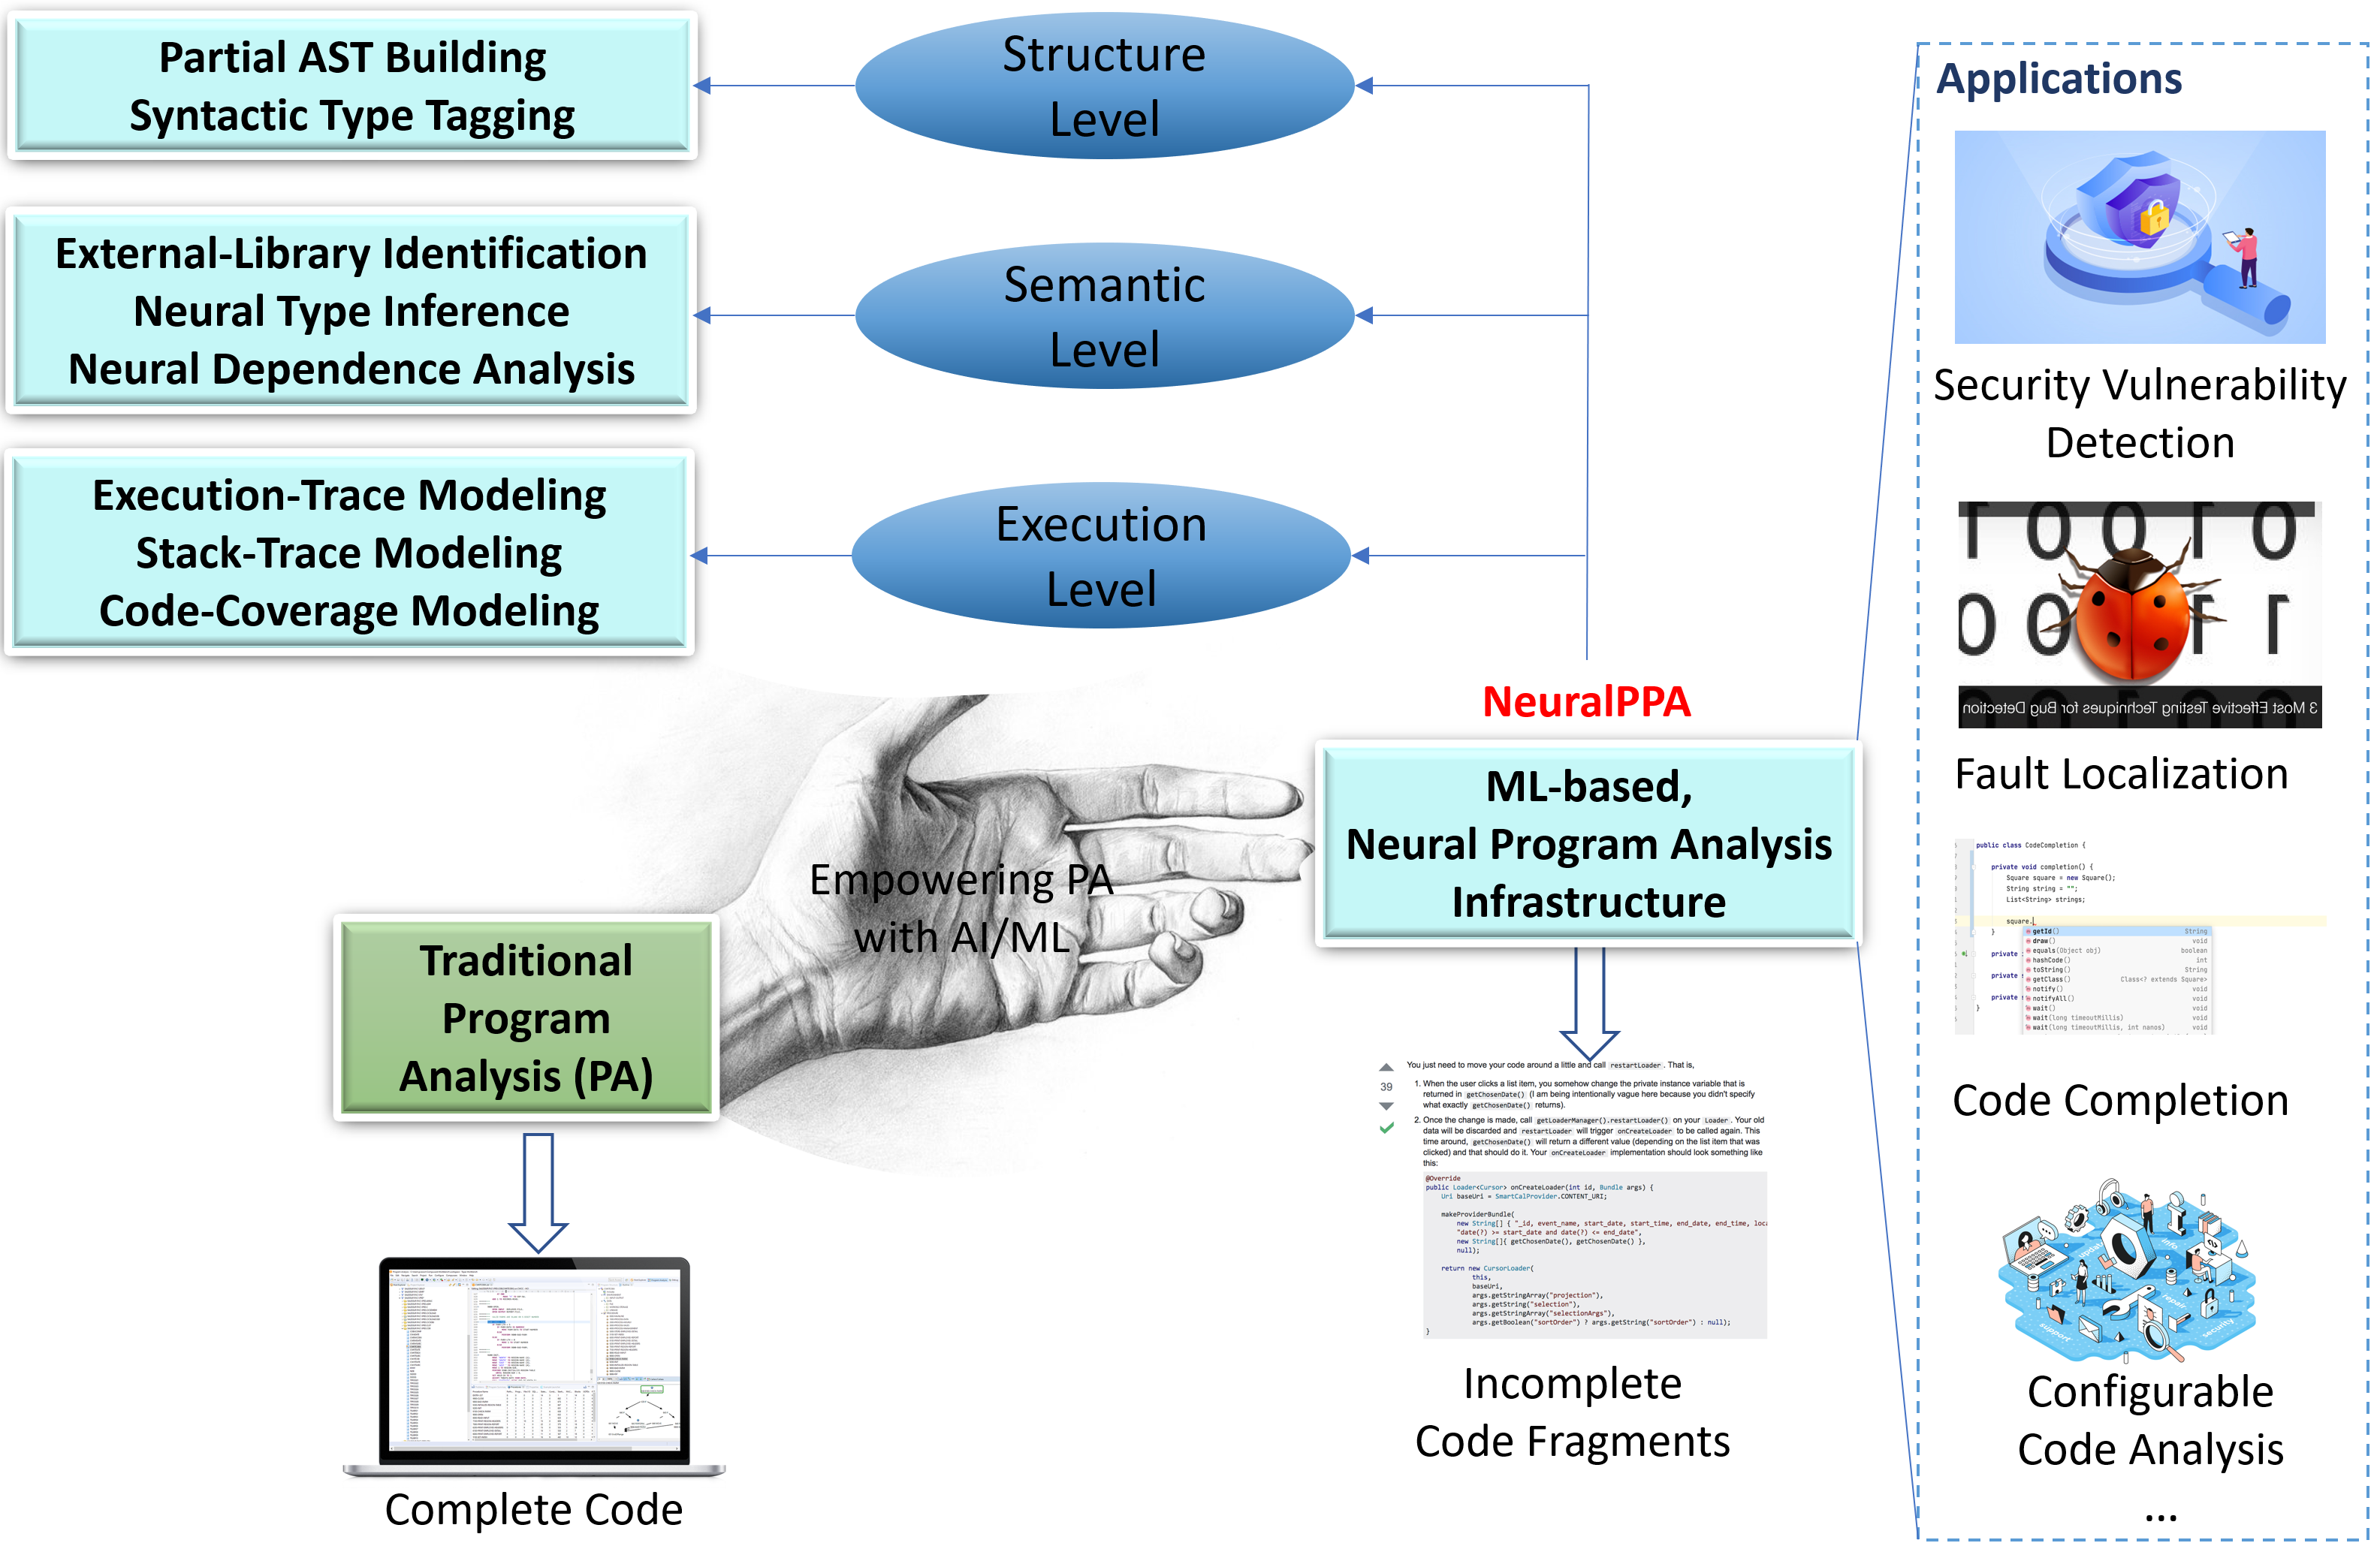
\includegraphics[width=0.83\textwidth]{graphs/neuralppa}
    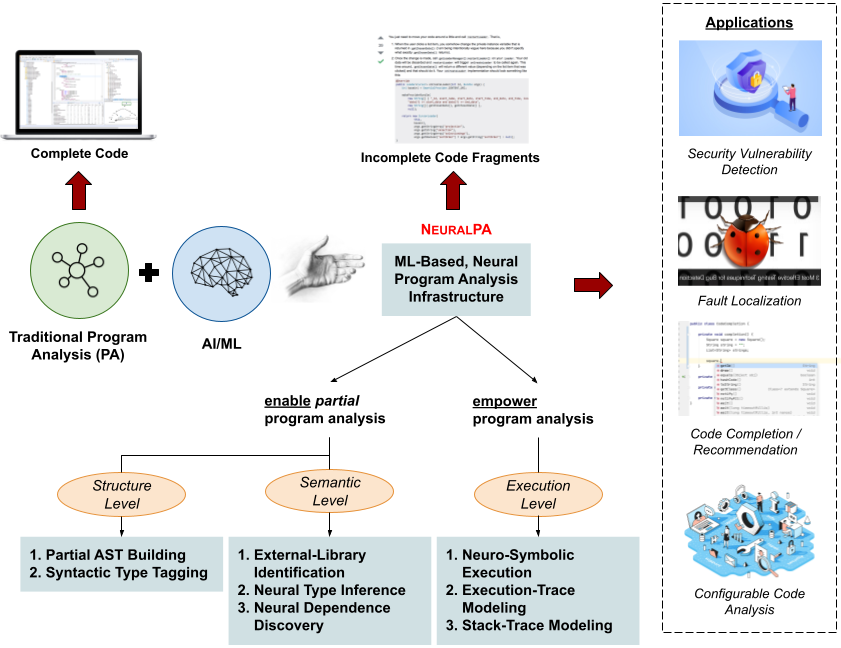
\includegraphics[width=0.92\textwidth]{figures/infra-design-3.png}
%    \vspace{-10pt}
    \caption{{\tool}: Machine Learning-based Program Analysis Infrastructure}
    \label{fig:arch}
\end{figure}


In this proposal, we seek to address these issues and advance the state-of-the-art in traditional program analysis by means of {\tool}, a {\em \underline{Neural} Network-Based \underline{P}rogram \underline{A}nalysis} infrastructure. We aim to establish {\em a scientific foundation, novel methodologies, frameworks, models, and algorithmic solutions for neural program analysis}. Our primary focus areas can be summarized as follows: 

%(1) {\bf Enabling analysis of incomplete code fragments}, i.e., partial program analysis;
(1) {\bf enabling analysis of incomplete code fragments}, i.e., partial program analysis;

%(2) {\bf Empowering existing PA tools by making them more sound and complete}. 
(2) {\bf empowering existing PA tools with advanced AI/ML
%techniques
} to make them more sound and complete.

\noindent Figure~\ref{fig:arch} illustrates the 
%general 
framework for {\tool}, which will allow the construction of efficient program analysis techniques for (partial) code, also based on which downstream 
%software engineering 
SE applications can be built.


\begin{center}
    \begin{minipage}{36em}
The key philosophy that drives our work is that the {\em structural, semantic, and symbolic execution-level analyses of partial code can be learned from the analysis of entire programs in the wealth of information obtained from ultra-large-scale, open-source software repositories}.
    \end{minipage}
\end{center}



We draw motivation for such a data-driven, learning-based approach from the following. First, ultra-large-scale software repositories, e.g., GitHub (7M+ projects) and SourceForge (700k+ projects), contain an enormous collection of programs. These repositories amount to 1B+ lines of code, 10M+ revision logs, and 3M+ issue reports. This wealth of knowledge is an excellent source for {\tool}. Hindle {\em et al.}~\cite{naturalness-icse12} have shown that code has high repetitiveness and predictability and can be captured well by statistical models. Thus, we expect to build ML/DL models to learn from those repositories. 
Second, the PI group reported a high repetitiveness level for AST code structure in open-source projects~\cite{icse15}. Thus, {\tool} infrastructure could help learn structure-level information from the ASTs extracted for whole programs in the existing code repositories and infer data types, partial ASTs for partial programs. Third, in an empirical study on the repetitiveness, containment, and composability of PDGs in open-source projects, the PI group~\cite{msr16} reported that among 17.5M PDGs with 1.6B PDG subgraphs, 14.3\% of the PDGs have all of their subgraphs repeated across different projects. Furthermore, in 15.6\% of the PDGs, at least 90\% of their subgraphs are likely to have appeared before in other projects. 
%Thus, {\tool} could learn from PDGs with complete program dependencies retrieved from existing code repositories and derive the dependencies for the (partial) code fragment under study. The PI group also reported a high repetitiveness level for AST code structure in open-source projects~\cite{icse15}.
Thus, {\tool} could learn semantic-level information from the PDGs with complete program dependencies retrieved from existing code repositories and infer such dependencies for the partial code fragment. Execution can also be modeled
from the ones in the past.

%\textcolor{red}{Add a line for execution-level}.

%Finally, such a program analysis infrastructure like {\tool} can be
%drawn from the spirit and successes of the approaches in natural
%language processing (NLP). For example, at the lexical level, the task
%of deriving the token types for source code tokens could be analogous
%to the part-of-speech (PoS) tagging in NLP. At the syntax level, the
%task of learning the syntactic structure in AST of the partial code
%can be inspired by the approaches to build parse trees for
%natural-language texts. At the semantic level, the partial program
%dependence analysis infrastructure is similar in spirit to the neural
%network-based dependency parsing in NLP, which learns the dependencies
%signifying the semantic relationships between words in a sentence from
%text corpora. In addition, there is much room for innovations in AI/ML
%for source code.

Broadly, the proposed program analysis infrastructure, \tool, draws inspiration from the successes of the neural network-based approaches in the field of natural language processing (NLP). For example, the task of deriving the data types for the source code tokens is analogous to the part-of-speech (POS) tagging task in NLP. At the syntactic level, learning the syntactic structure, i.e., the ASTs for partial code can be inspired by the approaches to infer parse trees for natural language texts. At the semantic level, the partial program dependence analysis infrastructure is similar in spirit to neural network-based dependency parsing in NLP, which learns the dependencies signifying the semantic relationships between words in a sentence from text corpora. In addition, there is much room for innovations in AI/ML for source code.


To accomplish these tasks, we propose the following thrusts of research in {\tool} (see Table~\ref{tab:milestones}):

\vspace{3pt}
%\noindent \textbf{Thrust 1. Neural Structural Analysis Infrastructure
%  \code{NeuralStruct}.} ({\em Section~\ref{}}) Source code has
%well-defined structures and semantics. Thus, the basic infrastructure
%in {\tool} is the neural structural analysis component.  This
%component has two main tasks. First, it learns from the syntactic
%structures of the complete code in the training dataset collected from
%large-scale code repositories, to derive the abstract syntax tree
%(AST) that best represents the syntactic structure of the given
%partial code, i.e., with the highest likelihood/probability.  The
%traditional lexical analyzer still works for partial code due to the
%independence nature of lexical tokens. The second task of this
%component is to tag the code tokens with the types of the syntactic
%units including the statement types (\code{if}, \code{for}, etc.),
%variables, fields, methods, classes, etc. Both of the tasks can be
%performed with our learning-based approaches in a dual-learning
%manner.

\noindent \textbf{Thrust 1. Neural Structural Analysis Infrastructure.} ({\em Section~\ref{sec:thrust1}}) Source code has a well-defined structure and semantics. Thus, the basic infrastructure in {\tool} is the neural structural analysis component, which primarily has two tasks. First, it learns from the syntactic structures of the complete code in the training dataset collected from large-scale code repositories, to derive the abstract syntax tree (AST) that best represents the syntactic structure of the given partial code, i.e., with the highest likelihood/probability. The traditional lexical analyzer still works for partial code due to the independence nature of lexical tokens. The second task of this component is to tag the code tokens with the types of the syntactic units including the statement types (\code{if}, \code{for}, etc.), variables, fields, methods, classes, etc. Both of the tasks can be performed with our learning-based approaches in a dual-learning manner.
  
\vspace{3pt}
\noindent \textbf{Thrust 2. Neural Semantic Analysis Infrastructure.}
({\em Section~\ref{sec:thrust2}}) The basis components for several
analysis techniques on the semantics of the program include the
following:

1) the identification of the APIs of the external libraries in the
external references in the partial code: this is needed because the
partial code contains the undeclared reference and/or
declaration/reference ambiguity without explicit declaration of the
APIs in the external libraries.

2) the inference of the type information for the entities in the
partial code: due to the ambiguity in the declaration, the types of
the variables and statements are not always obviously
identified. Thus, the type inference is a basic service within
{\tool}.

3) the inference of the program dependencies among the statements in
the partial code: several program analysis techniques are based on the
program dependencies, which are not always obtainable due to the
incompleteness of the given code fragment.

\vspace{3pt}
\noindent \textbf{Thrust 3. Neural Symbolic Execution Infrastructure.}
({\em Section~\ref{sec:thrust3}})
Symbolic execution is a means of analyzing a program to determine what
inputs cause each part of a program to execute. Symbolic execution
performs executing a program abstractly, so that one abstract
execution covers multiple possible inputs, which are assumed to have
symbolic values. We aim to explore the novel area in AI named
neuro-symbolic learning, which seeks to combine traditional
rules-based AI approaches with modern deep learning techniques.  We
will leverage traditional program analysis rules to enhance the
learning of the characteristics on the execution of the partial code
fragment.

\vspace{3pt}
\noindent \textbf{Thrust 4. Neural Partial Program Analysis
  Applications.}  ({\em Section~\ref{sec:thrust4}}) Our last thrust of research
is aimed to evaluate our basic partial program analysis infrastructure
in a few applications. The following software engineering
applications could be our examples: 1) software vulnerability detection for code snippets,
2) fault localization, and 3) code completion.

%\vspace{3pt}
%\noindent \textbf{Thrust ???. Neural Execution Analysis Infrastructure.}
%({\em Section~\ref{}}) All the dynamic analysis techniques require the
%analysis and understanding of the execution. However, for an
%incomplete code, we first need to design a component that can wrap
%around the given code fragment with the minimum code so that the code
%fragment can be executed. When the code is executed, we also need the
%approaches that represent the executed statements and their relations,
%model the execution and stack traces, and model the code coverages
%for an execution.


\begin{table*}[t]
	\vspace{-15pt}
\begin{center}
{\footnotesize{
\begin{tabular}{cc}
\begin{tabular}[t]{|p{0.2in}|p{2.95in}|} 
\hline
\multicolumn{2}{|>{\columncolor[gray]{0}}c|}{\textcolor{white}
{\bf Year 1 Project Milestones \& Deliverables}}\\
\hline 
\hline
\multicolumn{2}{|c|}{\bf T1. Neural Structure Analysis Infrastructure}\\
\hline
{\bf 1.1} & Neural Syntactic Type Tagging\\
{\bf 1.2} & Neural Partial AST Building\\
{\bf 1.3} & Evaluation of the components\\
\hline
\hline
\multicolumn{2}{|c|}{\bf T2. Neural Semantic Analysis Infrastructure}\\ 
\hline
{\bf 2.1} & External-Library Identification\\
\hline
%\hline
%\multicolumn{2}{|c|}{\bf Integrate Code Synthesis into Tools}\\
%\hline
%{\bf 1.5} & \goalOneFour.\\
%\hline
\multicolumn{2}{c}{}
\end{tabular}
&
\begin{tabular}[t]{|p{0.2in}|p{2.95in}|} \hline
\multicolumn{2}{|>{\columncolor[gray]{0}}c|}{\textcolor{white}
{\bf Year 2 Project Milestones \& Deliverables}}\\
\hline 
\hline
\multicolumn{2}{|c|}{\bf T2. Neural Semantic Analysis Infrastructure}\\
\hline
{\bf 2.2} & Neural Type Inference\\
{\bf 2.3} & Neural Dependence Analysis\\
%{\bf 2.3} & Integrate Evaluation Framework into Design Environment\\
%{\bf 2.4} & Evaluate CRL Framework with Existing Models\\
%{\bf 2.3} & \goalTwoThree.\\

\hline
\hline
\multicolumn{2}{|c|}{\bf T3. Neural Execution Analysis}\\ 
\hline
%{\bf 3.1} & Design New Code Representations and Learning Models.\\
{\bf 3.1} & Neural Execution-Trace Modeling\\
%{\bf 2.4} & Advance FL and RT-CI Approaches.\\
%{\bf 2.5} & Advance Regression Testing in CI Approaches.\\
%{\bf 2.5} & Advance APR Approaches with Framework.\\
\hline
%\hline
%\multicolumn{2}{|c|}{\bf Community Involvement: Capacity Building}\\
%\hline
%{\bf 2.4} & \goalTwoFour.\\
%{\bf 2.5} & \goalTwoFive.\\
%{\bf 2.6} & \goalTwoSix.\\
%\hline
\multicolumn{2}{c}{}
\end{tabular}
\end{tabular}\\
\vspace*{-.3cm}
\begin{tabular}{c}\hline
\multicolumn{1}{|>{\centering\columncolor[gray]{0}}p{6.44in}|}{\textcolor{white}
{\bf Year 3 Project Milestones \& Deliverables}}\\
\hline
\end{tabular}\\
\vspace*{-.2cm}
\begin{tabular}{cc}
\begin{tabular}[t]{|p{0.2in}|p{2.95in}|}
\hline
\multicolumn{2}{|c|}{\bf T3. Neural Execution Analysis}\\
\hline
{\bf 3.2} & Neural Stack Trace Modeling\\
{\bf 3.3} & Neural Code Coverage Modeling\\

%{\bf 3.3} & Testing on Models in IDE tools.\\
\hline
%\hline
%\multicolumn{2}{|c|}{\bf \goalTwo}\\ 
%\hline
%{\bf 3.3} & \goalThreeThree.\\
%\hline
\multicolumn{2}{c}{}
\end{tabular}
&
\begin{tabular}[t]{|p{0.2in}|p{2.95in}|}
\hline
\multicolumn{2}{|c|}{\bf T4. Neural Partial Program Analysis Applications}\\
\hline
%{\bf 3.1} & Design New Code Representations\\

{\bf 4.1} & Security Vulnerablity Detection with {\tool}\\
{\bf 4.2} & Fault Localization and Completion with {\tool}\\

\hline
\multicolumn{2}{c}{}
\end{tabular}
\end{tabular}
\vspace{-15pt}
}}
\end{center}
\vspace*{-.3in}
%\caption{Tasks and Milestones. (Rep. = Representation)}
\caption{The 3-year schedule of Thrusts, Tasks, and Milestones of this proposal.}
%the schedule of Thrusts, Tasks, and Milestones of this proposal.
%\vspace{-10pt}
\label{tab:milestones}
\vspace{-10pt}
\end{table*}
%


Toward this theme, in our preliminary work, we developed DeepPDA
(Section~\ref{sec:deeppda}), a neural network-based partial program
dependence analysis approach that learns to derive the program
dependencies for any code fragments (i.e., both complete and
incomplete). In our preliminary empirical evaluation, we intrinsically
evaluated it on Java and C/C++ programs. We trained DeepPDA on
complete code. For testing, we treated each method individually and
chose a consecutive portion within the method to predict the program
dependencies, and compared them against the actual
dependencies. Overall, DeepPDA predicts CFGs/PDGs in Java with
an F-score of 94.29\%, and in C++ with an F-score of 92.46\%. As
another preliminary work (Section~\ref{sec:statype}), we also
developed an approach to derive the data types of the variables in the
code snippets. We treat the problem as statistical machine translation
from source code with partially qualified names to source code with
full names. Our preliminary evaluation on StackOverflow posts shows
that our technique achieves high accuracy with 97.6\% precision and
96.7\% recall in deriving data types in code snippets.



%\subsection{Significance of This Proposed Project: NSF Merit Criteria}

\section{Intellectual Merits}

The results of this project will advance the state-of-the-art
knowledge and scientific foundations in both software security and
machine learning (explainable AI). They are transformative and
directly help improve software quality with novel automated software
vulnerability detection and assessment techniques.

\noindent \underline{{\bf Advance the state-of-the-art knowledge and
    understanding}}. Explainable AI-enabled vulnerability detection in
both binary and source code in Thrusts 1 and 3 will advance the body
of knowledge and theoretical foundations for both areas of machine
learning for code and software security. Thrust 2 will also help
advance the practical tools in software security and engineering.

\noindent \underline{{\bf Scientific foundation, creative/original
    research}}. This project will provide a scientific foundation
(novel concepts, representations, algorithms, models, and tools) (1)
to enable the explanations for ML models in vulnerability detection,
(2) to empower the ML-based vulnerability detection and assessment.

%and (3) to enable the applications of program analysis on incomplete
%code such as vulnerability detection on code snippets, code
%completion, etc.

\section{Broader Impacts}

\underline{{\bf (1) Transformative and benefits to society}}. Our
results will be transformative and directly benefit to our society.
They will lead to increasing software quality \& reliability, software
security.  Our validation involves students and professionals,
promoting teaching, training, and learning of both {\bf software
  security} and {\bf machine learning} techniques that have wide
impacts in industry and academic communities.

\noindent\underline{{\bf (2) Foster other related research
    activities}}. Our results will foster {\em research activities in
  related fields of {\bf explainable AI/ML} and {\bf software
    engineering}}. We will produce theoretical concepts and techniques
that are novel in deep learning, e.g., XAI model for source and binary
code. The applications of our techniques in software engineering
applications will advance software security and reliability.

%The collected {\bf large scale bug\&fix corpus} will be useful for
%software quality and reliability research.
%Innovations in CRL could be used to {\bf advance other SE tasks}. We
%will also develop {\bf novel DL-based bug detect-fix} approaches.


\noindent\underline{{\bf (3) Education, dissemination, and broader participation}} (Section~\ref{edu}). The
research will enhance the infrastructure for teaching/research via
tools and data sets for use by students and practitioners, and for
enhancement by researchers. We will provide related learning
modules for educators as well. It will include outreach activities for
undergraduate students, underrepresented groups, minorities, and women
in science.
%contribute novel
%teaching modules to our curriculum.
%Details will be presented in Section~\ref{edu}




\section{Related Work}
\label{sec:rw}

{\bf Vulnerability Detection.} Various techniques have been developed
to detect vulnerabilities.
%Security experts or researchers can utilize the fuzzing techniques~\cite{bohme2017coverage,wang2010taintscope,wen2020memlock,wang2017skyfire},
%symbolic execution~\cite{stephens2016driller,cha2015program,babic2011statically} or even manual auditing to hunt the vulnerabilities. However, the above approaches still require a large amount of time and resources to hunt the vulnerable code, even worse, most of the effort is wasted in analyzing the non-vulnerable code. Therefore, directly analyzing source code to identify the potential vulnerable code to help the vulnerability hunt is attracting a lot of attention.
%fuzzing (e.g., [9, 11, 39, 52, 63, 64, 67, 69, 70]), symbolic execution (e.g., [6, 10, 24, 60]) or manual auditing.
The rule-based approaches were developed to leverage known vulnerability patterns to discover possible vulnerable code, such as FlawFinder~\cite{FlawFinder}, RATS~\cite{RATS}, ITS4~\cite{viega2000its4}, Checkmarx~\cite{Checkmarx}, Fortify~\cite{HPFortify} and Coverity~\cite{Coverity}.
Typically, the patterns are manually defined by human experts. The state-of-the-art vulnerability detection tools using static analysis provide the
rules for each vulnerability type.
%For example,
%This category includes the lightweight methods that
%generate patterns from source code (e.g.,
%the well-known open source tools include FlawFinder~\cite{FlawFinder}, RATS~\cite{RATS}, ITS4~\cite{viega2000its4}, and the commercial tools include Checkmarx~\cite{Checkmarx}, Fortify~\cite{HPFortify} and Coverity~\cite{Coverity}.
%However, the rule-based approaches suffer the problem of high-false positives or high-false negatives and also more focus on one or few types of vulnerabilities.
%and the more comprehensive methods that
%generate patterns based on intermediate code (e.g., commercial
%tools Fortify~\cite{HPFortify} and Coverity~\cite{Coverity}).
%These tools can report
%the locations and the types of vulnerabilities, but cannot
%accurately distinguish between various vulnerable code and
%non-vulnerable code, resulting in high false positives or high
%false negatives~\cite{li2018vuldeepecker}.
Another type of VD approaches is machine learning (ML)-based.
%Tien
%Typically, these approaches require human-crafted or summarized
%metrics as features to characterize vulnerabilities and train machine
%learning models on the defined features to predict whether a given
%code is vulnerable or not.
%Traditional machine learning-based methods rely on human
%experts for defining features to characterize vulnerabilities,and use traditional machine learning techniques [37], such as k-nearest neighbor and support vector machine, to classify vulnerable code and non-vulnerable code.
%For example,
%Ghaffarian and Shahriari~\cite{ghaffarian2017software} [38] reviewed the approaches of vulnerability analysis and discovery using machine-learning techniques, most of which are traditional machine learning-based methods.
Various ML-based approaches have been built on top of distinct metrics, such as terms and their occurrence frequencies~\cite{scandariato2014predicting}, imports and function calls~\cite{neuhaus2007predicting}, complexity, code churn, and developer activity~\cite{shin2010evaluating}, dependency relation ~\cite{neuhaus2009beauty}, API symbols and subtrees~\cite{yamaguchi2012generalized, yamaguchi2011vulnerability}.

%Therefore, these approaches rely on human experts to manually define features, and cannot pin down the precise locations of vulnerabilities because programs are represented in some coarse-grained granularities.

%Attributes are the features that are defined to characterize pieces of code, including terms and their occurrence frequencies~\cite{scandariato2014predicting}, imports and function calls~\cite{neuhaus2007predicting}, complexity, code churn, and developer activity~\cite{shin2010evaluating}, dependency relation ~\cite{neuhaus2009beauty}, API symbols and subtrees~\cite{yamaguchi2012generalized, yamaguchi2011vulnerability}, system calls~\cite{grieco2016toward}, and the combination of some features above~\cite{chernis2018machine}. Therefore, these approaches rely on human experts to manually define features, and cannot pin down the precise locations of vulnerabilities because programs are represented in some coarse-grained granularities.
%Traditional machine learning-based methods can
%be characterized by the granularity and attributes. Granularity describes the ``atomic'' unit of code that is treated as a whole. Many granularities have been investigated, including program~\cite{grieco2016toward}, package~\cite{neuhaus2009beauty}, component~\cite{scandariato2014predicting, neuhaus2007predicting},
%file ~\cite{moshtari2016evaluating, shin2010evaluating}, and function~\cite{yamaguchi2012generalized,yamaguchi2011vulnerability, chernis2018machine}.
%Attributes are the features that are defined to characterize pieces of code, including terms and their occurrence frequencies~\cite{scandariato2014predicting}, imports and function calls~\cite{neuhaus2007predicting}, complexity, code churn, and developer activity~\cite{shin2010evaluating}, dependency relation ~\cite{neuhaus2009beauty}, API symbols and subtrees~\cite{yamaguchi2012generalized, yamaguchi2011vulnerability}, system calls~\cite{grieco2016toward}, and the combination of some features above~\cite{chernis2018machine}. Therefore, these approaches rely on human experts to manually define features, and cannot pin down the precise locations of vulnerabilities because programs are represented in some coarse-grained granularities.

Deep learning has been applied to detect
vulnerabilities.  For example, some approaches train a DL model on
different code representations to detect vulnerabilities, such as the
lexical representations of functions in a synthetic
codebase~\cite{harer2018learning}, code snippets related to
API calls to detect two types of
vulnerabilities~\cite{li2018vuldeepecker}, syntax-based,
semantics-based, and vector representations~\cite{li2018sysevr},
graph-based representations~\cite{zhou2019devign}.
%Harer et al.~\cite{harer2018learning} trained an RNN to detect vulnerabilities in .
%Lin et al.~\cite{lin2017poster} presented an approach to automatic learning high-level representations of functions based on their abstract syntax trees for vulnerability discovery.
%Russell et al. \cite{russell2018automated} proposed a large-scale function-level vulnerability detection system to learn deep feature representation of source code after lexical analysis. %It combined the neural feature representations of function source code with random forest as a classifier.
%Harer et al.~\cite{harer2018automated} used machine learning methods to perform the data-driven vulnerability detection, and compared the effectiveness of using the source code and the compiled code.
%Devign~\cite{zhou2019devign} learns a set of code semantic representations, 6 types of graphs, using graph neural networks to conduct graph-level classification.
%The granularity of above approaches is function-level involving large numbers of statements which are not related to vulnerabilities.
%VulDeePecker~\cite{li2018vuldeepecker} uses a recurrent neural network (RNN) trained on code snippets related to library/API function calls to detect two types of vulnerabilities.
%SySeVR ~\cite{li2018sysevr} is a deep learning-based framework which uses syntax-based, semantics-based, and vector representations to detect various types of vulnerabilities at the slice level.
%Therefore, they are coarse-grained and cannot pin down the precise locations of vulnerabilities.
%The recently proposed VulDeePecker~\cite{li2018vuldeepecker} is the first to use deep learning to detect vulnerabilities at the slice level (finer than function level), effectively excluding the statements which are not related to vulnerabilities.
%is a general graph neural network based model for graph-level classification through learning on a rich set of code semantic representations.
Some ML-based approaches could detect vulnerabilities from the binary
code including Genius~\cite{genius16}, Gimini~\cite{gimini17}, and
IoTSeeker~\cite{iotseeker21}. They are based on the graph
representations for the PDGs in the binary code. None of them is
designed to provide interpretations for a model in term of vulnerable
statements.

%Our {\tool} is different from all of the above approaches.

%The main goal of {\tool} is to add more intelligence assistance (IA)
%using a small graph of code statements, key variables, and CWE
%description to explain why a detection model reaches a prediction.

%Nevertheless, there is no systematic comparative study to show the quantitative
%impact of different factors on the effectiveness of vulnerability
%detection. The present study follows VulDeePecker and more specifically
%studies the impact of control dependency in the code
%gadget, the imbalanced data processing, and the neural networks
%on the deep learning-based vulnerability detection. As
%discussed above, the extension is based on a completely new
%implementation using an extended open source tool Joern,
%because a straightforward extension cannot accommodate
%new semantic information for VulDeePecker which is based
%on the commercial tool Checkmarx.


%\section{Related Work - NSA}
%\subsection{XAI}

{\bf Explainable AI}. A machine learning model typically runs
two distinct operations for learning and
classification~\cite{B16,DBLP:conf/icml/MengBK20,DBLP:conf/icml/MukherjeeYBS20,DBLP:conf/icml/NockM20}. Learners
are generally `trained' by being provided input data already
classified with an appropriate output. Then, based on the learned
data, the algorithm can produce classifications for new
inputs. Machine learning comes in different types, including
supervised and unsupervised learning, reinforcement learning and
neural networks
\cite{DBLP:journals/csur/MayerJ20,DBLP:journals/csur/VerbraekenWKKVR20,DBLP:journals/csur/ChenZZ0S020,DBLP:journals/csur/QianSWJLGPJYZRW20,DBLP:journals/csur/GuoCLH020,DBLP:journals/csur/LeCB20,DBLP:journals/comsur/OlowononiRL21}. Supervised
learning is where the learning occurs when the system is fed
pre-categorized or labelled training data. Unsupervised learning is
learning that occurs without labelled input data, allowing the
algorithm to find its own patterns within the data. These two types of
ML can also be used in conjunction with each other. Reinforcement
learning is another type of ML in which during the training process
feedback is provided to the system
\cite{DBLP:conf/icml/AgarwalS020,DBLP:conf/icml/0003KWGL20,DBLP:journals/comsur/LeiTZLZS20,DBLP:journals/csur/MendoncaZB19}. Several
approaches have used ML for vulnerability
detection~\cite{li2018vuldeepecker,zhou2019devign,li2018sysevr,russell2018automated,chakraborty2020deep}. One
of the key problems extant in ML is the inability of human users to
understand exactly how a model came to a determination
\cite{DBLP:journals/comsur/LeiTZLZS20}.
%XAI seeks to address this `black box' problem, where ML often makes
%decisions through methods which cannot be explained in specifics.
Dorin {\em et al.}~\cite{doran17} outline four categories of XAI based
on the interpretability present in an XAI model, namely: opaque
systems, interpretable systems, comprehensible systems, and truly
explainable systems.

\begin{itemize}

\item \emph{Opaque systems} are the ones in which the mechanisms/algorithms mapping input data to output data are not visible to the user~\cite{doran17}.
%These systems are often closed-source, developed by software
%manufacturers to be provided to clients to meet specific needs, and
  %proprietary in nature.
  Opacity in AI introduces challenges when informing
  decisions in the public sector, where there is greater requirement
  for transparent and justified decision making.

%If transparency in a system cannot be provided, then post-hoc explanations can be used to `justify the outputs in terms of rationalisations of the systems workings rather than trying to show the actual workings~\cite{Preece18}. Existing instances of AI’s use in digital forensics are generally opaque in nature and require validation by a user. Opaque AI assists in evidence discovery rather than interpretation. For example, a file may be flagged as being of interest but a digital forensic examiner must still examine the file’s contents/metadata to determine the validity of the AI’s classification. Further, no reasoning for the AI’s classification is provided.

\item In \emph{interpretable system}, the user cannot only see, but also study and understand how inputs are mathematically mapped to outputs~\cite{doran17}.
%The authors of~\cite{BARREDOARRIETA202082} further differentiate between interpretability - `the ability to explain or to provide meaning in terms understandable to a human', and understandability, for which transparency and interpretability are necessary.
%They also acknowledge that the audience of an AI’s output as a variable affecting its explainability. This is a significant factor that must be considered for models implemented within DF field, where technical information must be communicated to individuals with different technical background knowledge. Not only does the DF field requires that AI be transparent, but its decision making and reasoning capability must also be accurate and comprehensible for courts and can be explained during a court proceedings.
Interpretability can be provided through methods including, but not limited to, linear/logistic regression, generalised linear models, generalised additive models, decision trees, decision rules and the Rulefit algorithm~\cite{Molnar20}.

\item A \emph{comprehensible system} emits symbols along with its output that allows a user to relate inputs and their corresponding output properties~\cite{doran17}.% In these systems, different detected features of the input data act as keys to specific values that are added to the outputs to present pointers of features detected within the data to users.
These systems additionally provide a form of comment to their output, in contrast to just the output as given by an opaque system. This output can take the form of confidence scores, which introduce trust or contrastive information which provide insight~\cite{chari20}.
  %For a system to be explainable in a manner suitable in the DF field by being self-evidential, it must be both interpretable and comprehensible. Justification must be given for the system’s output, and those justifications must follow from the inputted data. When investigating applications of AI systems in digital forensics, the authors of~\cite{Const19} found that with suitable tools using new methods for visualising and explaining results of computed answerssuch as argumentation schemes, AI could be used `to explain the conclusions (and their proof) in a transparent, comprehensible and justified way'. It follows then that the digital forensics field requires a truly explainable AI system to address issues includingwait times, case load, and high data volume.
  
\item A \emph{truly XAI} system formulates a line of reasoning that explains the decision-making process of a model using human-understandable features of the input data~\cite{doran17}. Truly explainable AI makes use of knowledge bases which contextualises analysed data within the system and thus provides a mechanism through which individual findings can be deconstructed, in various forms, to provide a justification for the model’s interpretation that logically follows from the provided input data.

%The authors of~\cite{Wang19} emphasise that such models must be user-centric, highlighting that prior studies have failed to justify specific implementations of their lines of reasoning, while providing background on links between human reasoning and XAI systems. Further to this, systems must prioritise the needs of end users (e.g. different user groups within a specific industry, or different stakeholders within the legal system) to be trusted. Developers of these systems should work with individuals who will employ these systems or else risk creating systems that provide responses too obtuse or jargonistic to be interpretable~\cite{Miller17}. Finally, if the model's output can be validated through the use of logically consistent and self-generated justifications, the need for the transparency of the decision-making model to the user is reduced, but not eliminated, which could potentially allow software providers to protect proprietary technologies.
\end{itemize}

%In extended detection and response \cite{FirstbrookLawsonGartner2021}, it is necessary that decisions made by and with the assistance of AI-based tools can be justified and explained to a human. For example, the report prepared by the US President's Council of Advisors and Technology (PCAST) \cite{NationalDistrictAttorneysAssociationPCAST} revealed that forensic disciplines in the U.S. lacked ‘quality culture’  \cite[p.33]{NationalDistrictAttorneysAssociationPCAST} and that nearly all crime laboratories were closely tied up with the prosecution of cases. The report also highlighted that the US Supreme Court held that ‘the admissibility of scientific expert testimony depended on its scientific reliability’ \cite[p.41]{NationalDistrictAttorneysAssociationPCAST}, and  forensic processes need to stand up to scientific scrutiny by being repeatable, reproducible, and accurate. Ideally, any methodology should be objective with ‘precise definitions’ of ‘feature identification, comparison and matching’ \cite[p.48]{NationalDistrictAttorneysAssociationPCAST}. Since this is not possible, and ‘the black box in the examiner’s head cannot be examined directly for its foundational basis in science’, the authors stressed the need for empirical study of examiners’ performance in ‘black-box studies’ to determine a likelihood of error based on the generalised performance of the forensic analyst cohort  \cite[p.49]{NationalDistrictAttorneysAssociationPCAST}. A truly explainable AI with a rationalizable ‘black-box’ could provide greater confidence in subjective forensic methodologies, by being both transparent in process and providing justified and logical reasoning.

%The above discussion reinforces the importance of designing systems that maximize the practical use of XAI to further enhance triage and analysis of digital forensic evidence, and to improve the efficacy of human expert integration, for example  digital forensic analysis by facilitating the extraction of forensically sound pieces of evidence (also known as artifact) to assist vulnerability detection and mitigation in our proposed HXAI-VDIM (see Figures \ref{fig:overview} and \ref{fig:arch}).

%\input{satc22-approach}
\section{Proactive Software Vulnerability Detection with Explainable AI}
\label{sec:thrust1}

\subsection{Vulnerable Source Code Detection with Graph-based Convolution Network} \label{sec:vd}

\begin{figure}[!hbt]
    \centering
    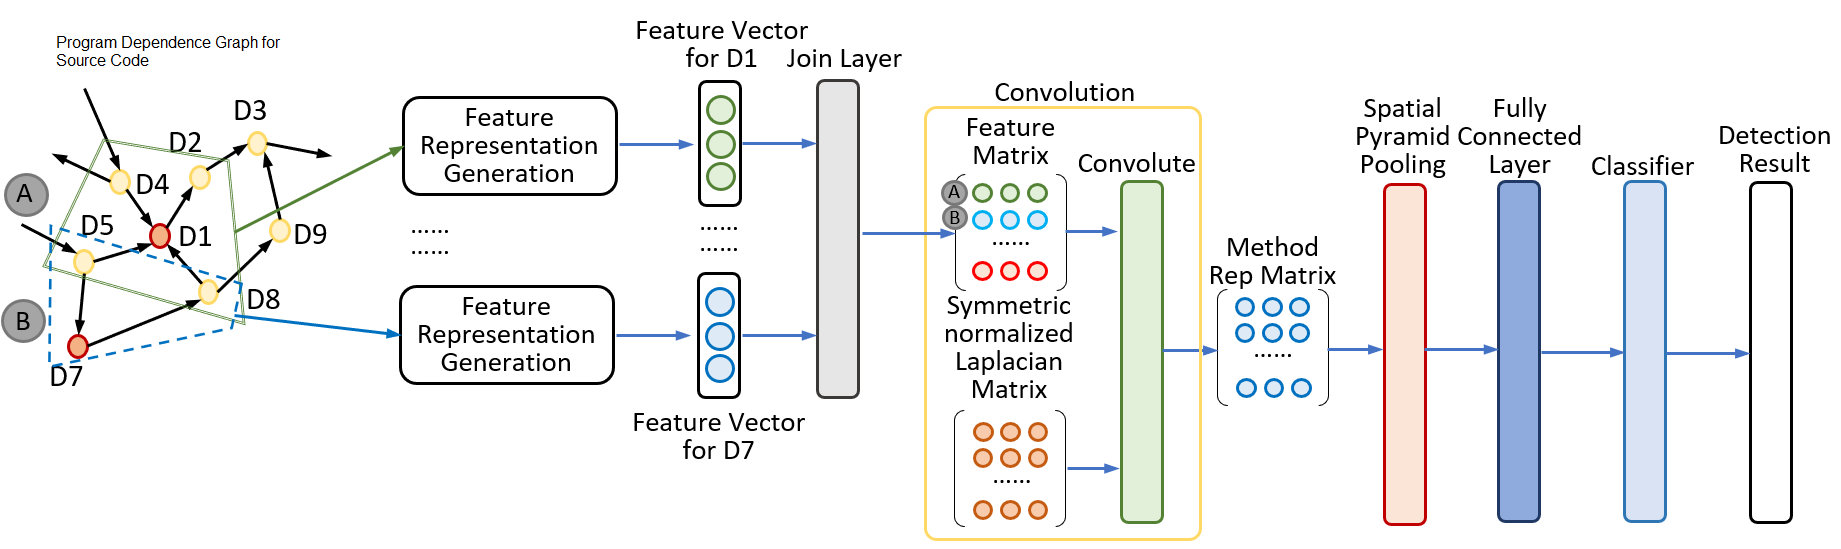
\includegraphics[width=6.5in]{graph-based-CNN.png}
    \caption{Feature-Attention, Graph-based Convolution Network for
      Vulnerability Detection Model}
    \label{fig:detection-model}
\end{figure}

Figure~\ref{fig:detection-model} shows our design of the Graph-based
Convolution Network (GCN) model for {\em proactive vulnerability
  detection at the source code level}. We also plan to use
Feature-Attention to enhance the GCN, and hereafter we will refer to
the model as FA-GCN. First, the source code under investigation will
be parsed and the program dependence graph (PDG) is extracted.  For
example, in Figure~\ref{fig:detection-model}, D1-D9 represent the
statements in a program under investigation. The edges represent the
control and data dependencies among the statements. For each
statement, we can use any set of features/attributes that are
important to the statements.
%Each node can be associated with attributes.

%devices in an IoT system are modeled as the nodes in a graph structure
%in a GCN. D1-D9 in Figure~\ref{fig:detection-model} are nine example
%IoT devices under study in the system, where the attributes and
%features of a node represent the properties associated with the IoT
%devices.

Similar to CNN using the filter on an image, FA-GCN performs sliding a
small window along all nodes (statements) of the PDG. For example, in
Figure~\ref{fig:detection-model}, the window marked with \circled{A}
for the node $D1$ consists of itself and the neighboring
statements/nodes $D2$, $D4$, $D5$, and $D8$. Another window (marked
with \circled{B}) is for the node $D7$ at the center, including itself
and the neighboring nodes: $D5$ and $D8$. For each window, FA-GCN
generates the feature representation matrix for the statement at the
center. For example, for the window centered at $D1$, it generates the
feature vector $F_{D1}$ for the statement $D1$. 

From the representation vectors for all statements, FA-GCN uses a join
layer to link all these vectors into the Feature Matrix
$\mathcal{F}_{m}$ for method $M$. A row in $\mathcal{F}_m$ corresponds
to a window in the input PDG graph.  Next, FA-GCN performs the
convolution operation by first calculating the symmetric normalized
Laplacian matrix~$\tilde{A}$~\cite{GCN16}, and then calculating the
convolution to generate the representation matrix $M_{m}$ for the
subset $S$ of the source code under investigation. After that, we use
the traditional steps as in a CNN model: using a spatial pyramid
pooling layer (to normalize the method representation matrix into a
uniform size, and reduce its total size), and connecting its output to
a fully connected layer to transform the matrix into a vector $V_S$ to
represent the subset $S$ of the IoT devices under study. With $V_S$,
we perform classification by using two hidden layers (controlling the
length of vectors and output) and a softmax function to produce a
prediction score for $S$. We use those scores as {\em vulnerability
  scores to rank the potentially vulnerable code}. The decision for
$m$ as vulnerable or not can be done via a trainable threshold on the
prediction score~\cite{li2018vuldeepecker,li2019improving}. The
detection results in terms of the scores for all statements are
recorded.

%Let us revisit {\em example scenario 1} presented in Section \ref{section:An Example Use Case}, where we assume that IoT devices and computation within them, particularly those that are publicly located within the campus network, can be compromised and used to facilitate other malicious cyber activities. 
% To model this scenario, each node in the FA-GCN model represents an IoT device (e.g., nodes for servers, smartTV, networks, camera, etc.), and the edges represent the interconnections among the devices. To train the FA-GCN, we can use the historical data from the same or similar IoT systems with their devices in the same device category. The data acquisition process is explained in Section~\ref{subsection:Data Acquisition}.

For training, the Vulnerability databases, e.g., Common
Vulnerabilities and Exposures in the National Vulnerability Database
(NVD) can also be used for training the vulnerability detection model.

%\noindent {\bf Risk Scanning Component}. A similar architecture can be used for the risk scanning component in an IoT system. In this case, the input graph is used to represent the connection structures among IoT devices. The attributes of the nodes represent the features and the {\em risk scores for the IoT devices}. To train the model to evaluate the risk scores, we can rely on the historical data of the devices over time. 

\subsection{Explainable AI for Vulnerability Detection}
\label{sec:xai}

\begin{figure}[!hbt]
    \centering
    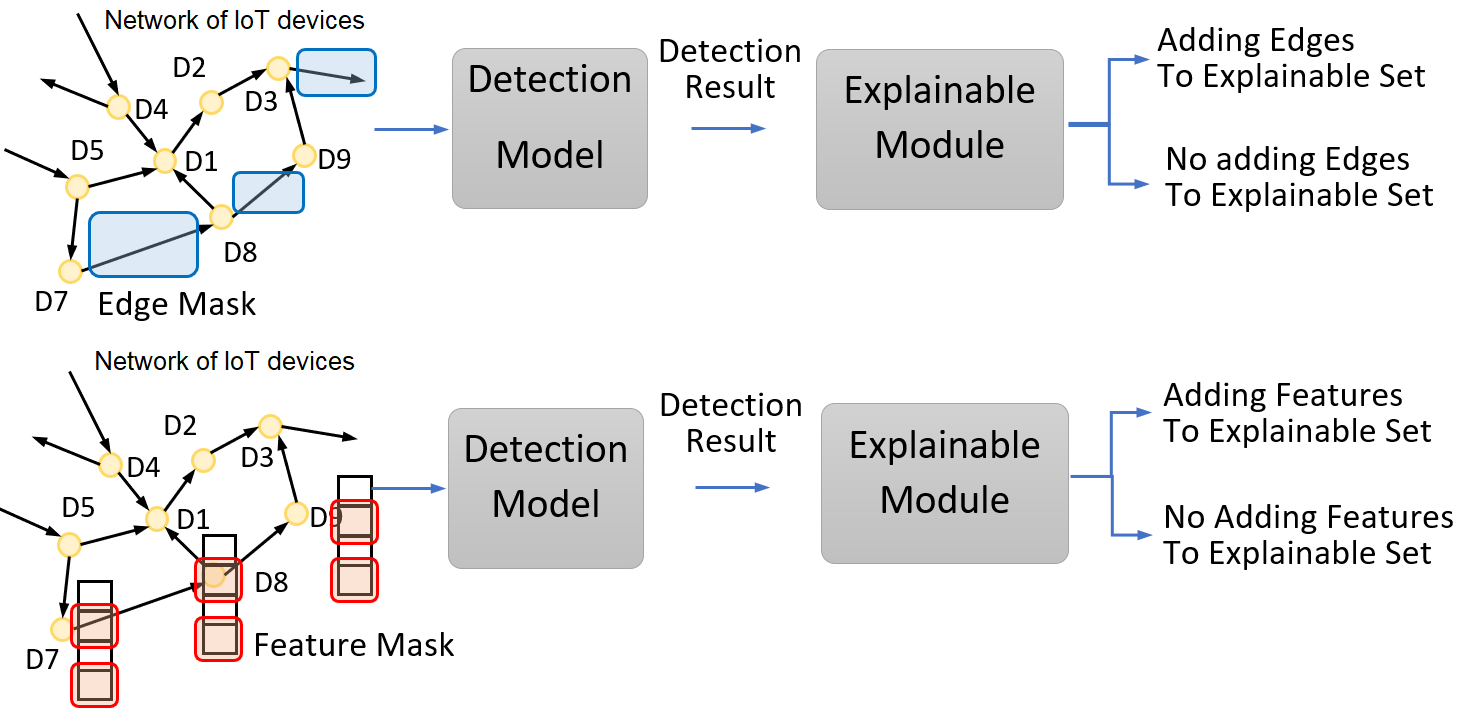
\includegraphics[width=3.8in]{xai-example.png}
    \caption{Graph-based Explainable Model for Vulnerability Detection}
    \label{fig:xai}
\end{figure}

%After each iteration of the detection, it is not necessarily that the detected vulnerable devices at this iteration are  the correct ones. Therefore, we integrate the human expert and analyst in the loop. We then

The explainable AI model takes the detection result with the
vulnerability scores for all the statements and the FA-GCN detection
model itself to produce the {\bf Explainable Set}, {\em which is
  defined as the set containing the parts of the input explaining the
  reason for the model to decide the detected
  vulnerability}. Specifically, it uses both the input graph $G_M$ of
the PDG and the FA-GCN model as the input to obtain the Explainable
Set.
To that end, our goal is to take the FA-GCN and a specific input graph
$G_M$ for PDG of the code under study, and produce the {\em crucial
  sub-graph structures} and {\em crucial features} in $G_M$ that
affect the decision of the FA-GCN detection model.

We leverage our preliminary work on XAI~\cite{fse21-submission}: our
idea is that {\em if removing or altering a node or a feature in the
  input PDG graph of the code does affect much the prediction scores,
  the node or the feature is considered as essential and thus must be
  included in the explainable set}. We use
GNNEXplainer~\cite{GNNExplainer} as follows. It searches for a
sub-graph $\mathcal{G}_M$ in $G_M$ that minimizes the difference in
the prediction scores between using the whole graph $G_M$ and the
minimal graph $\mathcal{G}_M$. Without that subgraph $\mathcal{G}_M$
in the input $G_M$, the model would not decide $G_M$ as vulnerable,
thus, $\mathcal{G}_M$ is considered as {\bf crucial PDG sub-graph}
consisting of {\bf crucial features} in those statements and
connections {\bf relevant to the detected vulnerability}.

\noindent {\em Potential Impacts of Explanations}.  The
statements with crucial features in both Explainable Sets will be
visualized and presented to the security expert. Based on his/her
expertise, (s)he can quickly omit the benign code from the list of
potentially vulnerable code.

%Correctly detected vulnerable device(s) will be isolated and prevented
%from further interaction in the network (i.e., no sending or receiving
%data). The input graph representing the adjusted IoT system with the
%new graph structure of IoT devices will be the input for the next
%iteration of detection.

%Let us revisit {\em example scenario 1} in Section~\ref{section:An Example Use Case} again. Assume that after the first iteration, the model detects that nodes corresponding to servers A, B, and C, router D,  camera E, and  smart TV F are vulnerable. However, with the expertise and knowledge from the expert, router D, which cannot be accessed from the outside, can be quickly eliminated from the suspicious list. The model in the next iteration will not consider router D in the detection process and its parameters will be updated accordingly. The process will continue with the integration of human experts in the loop.
   

\noindent \underline{\bf Formulation.}  Let us formulate how we build
the explainable sets and features/attributes. The input includes the
trained FA-GCN model, the input ($G_M$), and the detection scores for
all the nodes. Figure~\ref{fig:xai} illustrates our
algorithm to train the model.

To derive the explainable sets, the key goal is to find a sub-graph
$\mathcal{G}_M$ in the input $G_M$ that minimizes the
difference in the prediction scores between using the entire graph
$G_M$ and using the minimal graph $\mathcal{G}_M$. To do so, we use
GNNExplainer's {\em masking technique}~\cite{GNNExplainer},
which treats the searching for the minimal graph $\mathcal{G}_M$ as a
learning problem of the {\em edge-mask} set $EM$ of the edges,
and the {\em feature-mask} set $XM$ of the features.
The idea is that learning these two sets $EM$ and $XM$
helps {\tool} derive the explainable sub-graph $\mathcal{G}_M$
and the set of crucial feature $\mathcal{X}_M$
by masking-out the edges in $EM$
and the feature in~$XM$ from $G_M$ (input graph) and $F_M$ (input feature)
({\em Note}: ``masked-out'' is denoted by $\bigodot$):
\begin{equation}\label{eq:11}
\mathcal{G}_M = G_M \bigodot EM
\end{equation}
\begin{equation}
\mathcal{F}_M = F_M \bigodot XM
\end{equation}
In Figure~\ref{fig:xai}, the explainable module checks if the FA-GCN model produces the same result (in this case the result is
vulnerable). If yes, the edge in the edge-mask is not important and
is not included in $\mathcal{G}_M$. Otherwise, the edge is important
and included in $\mathcal{G}_M$.
Similar treatment is for {\em feature-mask} $XM$. In
Figure~\ref{fig:xai}, $FM$ masks the second and fourth features for
each node (IoT device) (Each device has the same number of
features).
Because the numbers of possible sub-graphs and the edge-mask sets
and feature-mask
are untractable, GNNExplainer uses a learning approach for the
edge-mask $EM$ and feature mask $XM$.

Let us formally explain how it works. It
formulates the problem by maximizing the mutual information (MI)
between the minimal graph $\mathcal{G}_M$ and the input~$G_M$:
\begin{equation}\label{maineq}
\max_{\mathcal{G}_M} MI(Y,\mathcal{G}_M, \mathcal{X}_M) = H(Y) - H(Y|G=\mathcal{G}_M, F=\mathcal{X}_M)
\end{equation}
$Y$ is the outcome decision by the FA-GCN model. Thus, the entropy term
$H(Y)$ is constant for the trained FA-GCN model. Maximizing the $MI$
value for all $\mathcal{G}_M$ and $\mathcal{X}_M$ is equivalent to minimizing conditional
entropy $H(Y|G=\mathcal{G}_M, X|F=\mathcal{X}_M)$, which by definition of
conditional entropy can be expressed~as
\begin{equation}
  \label{eq2}
-\mathbb{E}_{Y|\mathcal{G}_M}
  [log P_{FA-GCN} (Y|G=\mathcal{G}_M,F=\mathcal{X}_M)
  \end{equation}
The meaning of this conditional entropy formula is a measure of how
much uncertainty remains about the outcome $Y$ when we know
$G=\mathcal{G}_M$ and $F=\mathcal{X}_M$. GNNEXplainer also limits the
size of $\mathcal{G}_M$ by $K_M$, i.e., taking $K_M$ edges that give
the highest mutual information with the prediction outcome $Y$.
%
Direct optimization of the formula~\ref{eq2} is not tractable, thus,
we can treat $\mathcal{G}_M$ as a random graph variable
$\mathcal{G}$. The objective in Equation~\ref{eq2} becomes:
\begin{equation}
  \label{eq3}
  \min_{\mathcal{G}} \mathbb{E}_{\mathcal{G}_M \sim \mathcal{G}} H(Y|G=\mathcal{G}_M,F=\mathcal{X}_M)
\end{equation}
\begin{equation}
  \label{eq4}
  \min_{\mathcal{G}} H(Y| G=\mathbb{E}_{\mathcal{G}}[\mathcal{G}_M], F = \mathbb{E}_{\mathcal{X}}[\mathcal{X}_M])
\end{equation}
From Equation~\ref{eq3}, we obtain Equation~\ref{eq4} with Jensen's
inequality.  The conditional entropy in Equation~\ref{eq4} can be
optimized by replacing $\mathbb{E}_{\mathcal{G}}[\mathcal{G}_M]$ to be
optimized by masking with $EM$ on the input graph $G_M$.
Now, we can reduce the problem to learning the mask $EM$.
Similar treatment is applied to $XM$.
Details on training can be found in~\cite{GNNExplainer}. The resulting
sub-graph $\mathcal{G}_M$ is directly used as an explainable set. The resulting sub-set of feature $\mathcal{X}_M$ is also an explainable set.

The philosophy is to use Artificial Intelligence (AI) to detect the vulnerability, while using
Intelligence Assistant (IA) by providing explanations for
to support developers in further investigation.

\section{Thrust 2: Explainable AI-enabled Software Vulnerability Assessment}
\label{sec:thrust2}

\subsection{Motivating Example}
\label{exe:sec}

%CVE-2021-37714: description
%CVSS Scores

%Input-Output

%Code Change: src/main/java/org/jsoup/parser/HtmlTreeBuilder.java

%Crash-point or infinite loop: HtmlTreeBuilderState.java


Let us present an example from an HTML parser,~named {\em
  jsoup}, and our observations.
%for motivation.
Fig.~\ref{CVSS-tab} displays the information on the vulnerability
CVE-2021-37714 that was reported on {\em jsoup}, and published on
08/18/21.~The change that was deemed to contribute to the
vulnerability were committed at version 1.12.1 to the method
\code{process(Token,HtmlTreeBuilder)} of the
\code{Html\-Tree\-Builder\-State} class (lines 10--11, and 12 of
Fig.~\ref{fig:motiv-code}). That change directly uses the value
returned from \code{reset\-Inser\-tion\-Mode()} as the condition to
insert \code{starTag} (line 13). With this~change, certain input HTML
code with a specific start tag could make the program go to line 16
with a recursive call to the method \code{process(...)}. That~call
resulted in an NullPointerException at line 3 as noted in the
log:~{\em ``java.\-lang.\-Null\-Pointer\-Ex\-ception: Cannot invoke
  "org.\-jsoup.\-nodes.\-Element.\-normalName()" because the return
  value of
  "org.\-jsoup.\-parser.\-HtmlTree\-Builder.\-current\-Element()" is
  null.''}. In other cases, the parser can get stuck, i.e., {\em
  ``loop indefinitely until canceled''} as described in CVE-2021-37714 (Fig.~\ref{CVSS-tab}). Due
to those effects, this vulnerability is considered as {\em a denial of
  service (DoS)}.

\begin{figure}[t]
  \begin{flushleft}
    \footnotesize
\textbf{Vulnerability Details: CVE-2021-37714}\\
\textbf{1. Description}:
{\em jsoup is a Java library for working with HTML. Those using jsoup versions prior to 1.14.2 to parse untrusted HTML or XML may be vulnerable to DOS attacks. If the parser is run on user supplied input, an attacker may supply content that causes the parser to get stuck (loop indefinitely until cancelled), to complete more slowly than usual, or to throw an unexpected exception. This effect may support a denial of service attack. The issue is patched in version 1.14.2. There are a few available workarounds. Users may rate limit input parsing, limit the size of inputs based on system resources, and/or implement thread watchdogs to cap and timeout parse runtimes.
  Publish Date : 2021-08-18 Last Update Date : 2022-02-07}
%\textbf{2. Vulnerability Type(s)}: Denial Of Service
%{\bf 3. CVSS Score:} ...\\
%{\bf 4. Detailed CVSS Grades:}\\
\end{flushleft}
%  \centering
%  \tabcolsep 3pt
%  \scriptsize
%  \begin{tabular}{lll}
%   Vulner. Assess. Type   & Value & Description \\
%      \hline
%    Confidentiality Impact & {\bf None}  & No impact to the confidentiality \\
%    Integrity Impact & {\bf None}  & No impact to the integrity \\
%    Availability Impact & {\bf Partial} & There is reduced performance or\\
%    & & interruptions in availability\\
%    Access Complexity & {\bf Low} & Specialized access conditions or \\
%    & & extenuating circumstances do not exist\\
%    & & Little knowledge is required to exploit\\
%    Authentication & {\bf Not Req} & Authentication is not required \\
%    & & to exploit the vulnerability\\
%    Gained Access & {\bf None}  & No gained access with the vulnerability \\
%    Acccess Vector & {\bf Local} & The vulnerability is in the local parser \\
%    \end{tabular}%
  %  \label{CVSS:tab}%
  \vspace{-16pt}
\caption{Vulnerability Details: CVE-2021-37714}
\label{CVSS-tab}
\end{figure}

%\begin{wrapfigure}{l}{0.5\textwidth}
%	\centering
%	\lstset{
%		numbers=left,
%		numberstyle= \tiny,
%		keywordstyle= \color{blue!70},
%		commentstyle= \color{red!50!green!50!blue!50},
%		frame=shadowbox,
%		rulesepcolor= \color{red!20!green!20!blue!20} ,
%		xleftmargin=1.5em,xrightmargin=0em, aboveskip=1em,
%		framexleftmargin=1.7em,
%                numbersep= 5pt,
%		language=Java,
%    basicstyle=\tiny\ttfamily,
%    numberstyle=\tiny\ttfamily,
%    emphstyle=\bfseries,
%                moredelim=**[is][\color{red}]{@}{@},
%		escapeinside= {(*@}{@*)}
%	}
%	\begin{lstlisting}[]
%// .../jsoup/parser/HtmlTreeBuilderState.java
%boolean process(Token t, HtmlTreeBuilder tb) { ...
%  if (t.isCharacter()&& inSorted( (*@{\color{red}{tb.currentElement().normalName()}@*),InTableFoster)){
%     ...
%     return tb.process(t);
%  }
%  ...
%  } else {
%      tb.popStackToClose(name);
%(*@{\color{orange}{- \quad \quad tb.resetInsertionMode();}@*)
%(*@{\color{orange}{- \quad \quad if (tb.state() == InTable) \{}@*)
%(*@{\color{cyan}{+ \quad \quad if (!tb.resetInsertionMode()) \{}@*)
%         tb.insert(startTag);
%         return true;
%      }
%(*@{\color{red}{\quad \quad \quad return tb.process(t, InHead);}@*)
%      ...
%}
%	\end{lstlisting}
%        \vspace{-15pt}
%        \caption{Code Change at Version 1.12.1 for CVE-2021-37714}
%        \vspace{-6pt}
%        \label{fig:motiv-code}
%\end{wrapfigure}

%     tb.newPendingTableCharacters();
%     tb.markInsertionMode();
%     tb.transition(InTableText);


%vulnerability}.

Fig.~\ref{cvss} shows the Common Vulnerability Scoring System
grades (CVSS) given by security experts for
different \underline{v}ulnerability \underline{a}ssessment
\underline{t}ypes (VATs) for CVE-2021-37714. Due to the above effects,
the availability impact for this~vulnerability is rated as {\em
  Partial} (i.e., for some inputs, there will be reduced performance
and interruptions in available services).

%Recent research~\cite{deepCVA-ase21} has developed a machine learning
%(ML) model that learns from the existing grading from security experts
%to provide the new grading for a committed code change that was deemed
%to be vulnerable. This type of commit-level automated vulnerability
%assessment together with a vulnerability detection (VD) tool are very
%useful in helping developers to early detect and assess the impacts of
%the detected vulnerability as soon as the code is committed.  However,
%the state-of-the-art approach for commit-level vulnerability
%assessment is still limited as explained in the following
%observations.

\begin{figure}
     \centering
     \begin{minipage}{0.45\textwidth}
\centering
\lstset{
		numbers=left,
		numberstyle= \tiny,
		keywordstyle= \color{blue!70},
		commentstyle= \color{red!50!green!50!blue!50},
		frame=shadowbox,
		rulesepcolor= \color{red!20!green!20!blue!20} ,
		xleftmargin=1.5em,xrightmargin=0em, aboveskip=1em,
		framexleftmargin=1.7em,
                numbersep= 5pt,
		language=Java,
    basicstyle=\tiny\ttfamily,
    numberstyle=\tiny\ttfamily,
    emphstyle=\bfseries,
                moredelim=**[is][\color{red}]{@}{@},
		escapeinside= {(*@}{@*)}
	}
	\begin{lstlisting}[]
// .../jsoup/parser/HtmlTreeBuilderState.java
boolean process(Token t, HtmlTreeBuilder tb) { ...
  if (t.isCharacter()&& inSorted( (*@{\color{red}{tb.currentElement().normalName()}@*),InTableFoster)){
     ...
     return tb.process(t);
  }
  ...
  } else {
      tb.popStackToClose(name);
(*@{\color{orange}{- \quad \quad tb.resetInsertionMode();}@*)
(*@{\color{orange}{- \quad \quad if (tb.state() == InTable) \{}@*)
(*@{\color{cyan}{+ \quad \quad if (!tb.resetInsertionMode()) \{}@*)
         tb.insert(startTag);
         return true;
      }
(*@{\color{red}{\quad \quad \quad return tb.process(t, InHead);}@*)
      ...
}
	\end{lstlisting}
         \caption{Code Change v1.12.1 for CVE-2021-37714}
         \label{fig:motiv-code}
     \end{minipage}
     \hfill
     \begin{minipage}{0.5\textwidth}
%          \centering
%\textbf{2. Vulnerability Type(s)}: Denial Of Service

%{\bf 3. CVSS Score:} ...\\

%{\bf 4. Detailed CVSS Grades:}\\
       %  \centering
       \begin{flushleft}
  \tabcolsep 3pt
  \scriptsize
  \begin{tabular}{lll}
   Vulner. Assess. Type   & Value & Description \\
      \hline
    Confidentiality Impact & {\bf None}  & No impact to the confidentiality \\
    Integrity Impact & {\bf None}  & No impact to the integrity \\
    Availability Impact & {\bf Partial} & There is reduced performance or\\
    & & interruptions in availability\\
    Access Complexity & {\bf Low} & Specialized access conditions or \\
    & & extenuating circumstances do not exist\\
    & & Little knowledge is required to exploit\\
    Authentication & {\bf Not Req} & Authentication is not required \\
    & & to exploit the vulnerability\\
    Gained Access & {\bf None}  & No gained access with the vulnerability \\
    Acccess Vector & {\bf Local} & The vulnerability is in the local parser \\
  \end{tabular}%
  \end{flushleft}
    \caption{Detailed CVSS Impact Grades}
         \label{cvss}
     \end{minipage}
\end{figure}

\subsection{Proposed Solution}
\label{overview:sec}



%Figure~\ref{fig:overview} illustrates the overall architecture of
%{\tool}.

\noindent {\tool} has three key components working in three~steps
(Fig.~\ref{fig:overview}).

%\subsubsection*{{\bf Step 1. Multi-version PDG ({\mvpdgxy}) Generation}}

\vspace{2pt}
\subsubsection*{{\bf Step 1. Representing Code Changes and Contexts with Multi-version PDG ({\mvpdgxy})}}
Program Dependence Graph~\cite{pdg} is a directed graph with a
set $N$ of nodes and a set $E$ of edges. A node $n \in N$
represents a program statement or a conditional expression; an edge $e
\in E$ represents the data or control flow among the statements.
A graph representation, called multi-version program
dependence graph ({\mvpdgxy})~\cite{flexeme-fse20} represents the
code changes between two versions $x$ and $y$, before and after the
commit. 

\begin{Definition}[Multi-version Program Dependence Graph] ({\bf {\mvpdgxy}}).
A {\mvpdgxy}~\cite{flexeme-fse20} is a directed graph generated from the
disjoint union of all nodes and edges in the PDGs at versions $x$
and~$y$.
\end{Definition}

%{\mvpdgxy} is a directed graph generated from the disjoint union of
%all nodes and edges in both PDGs at the version $x$ and the version
%$y$ (Figure~\ref{fig:multi-version-pdg}).

%{\mvpdgxy} allows us to capture the program dependencies including data/control
%flows that are crucial in assessing the impacts of a vulnerability.

%Contextualized Embeddings for Code Changes



\vspace{2pt}
\subsubsection*{{\bf Step 2. Graph-based Representation Learning to build Contextualized Embeddings for Code Changes}}

\begin{wrapfigure}{l}{0.5\textwidth}
	\centering
	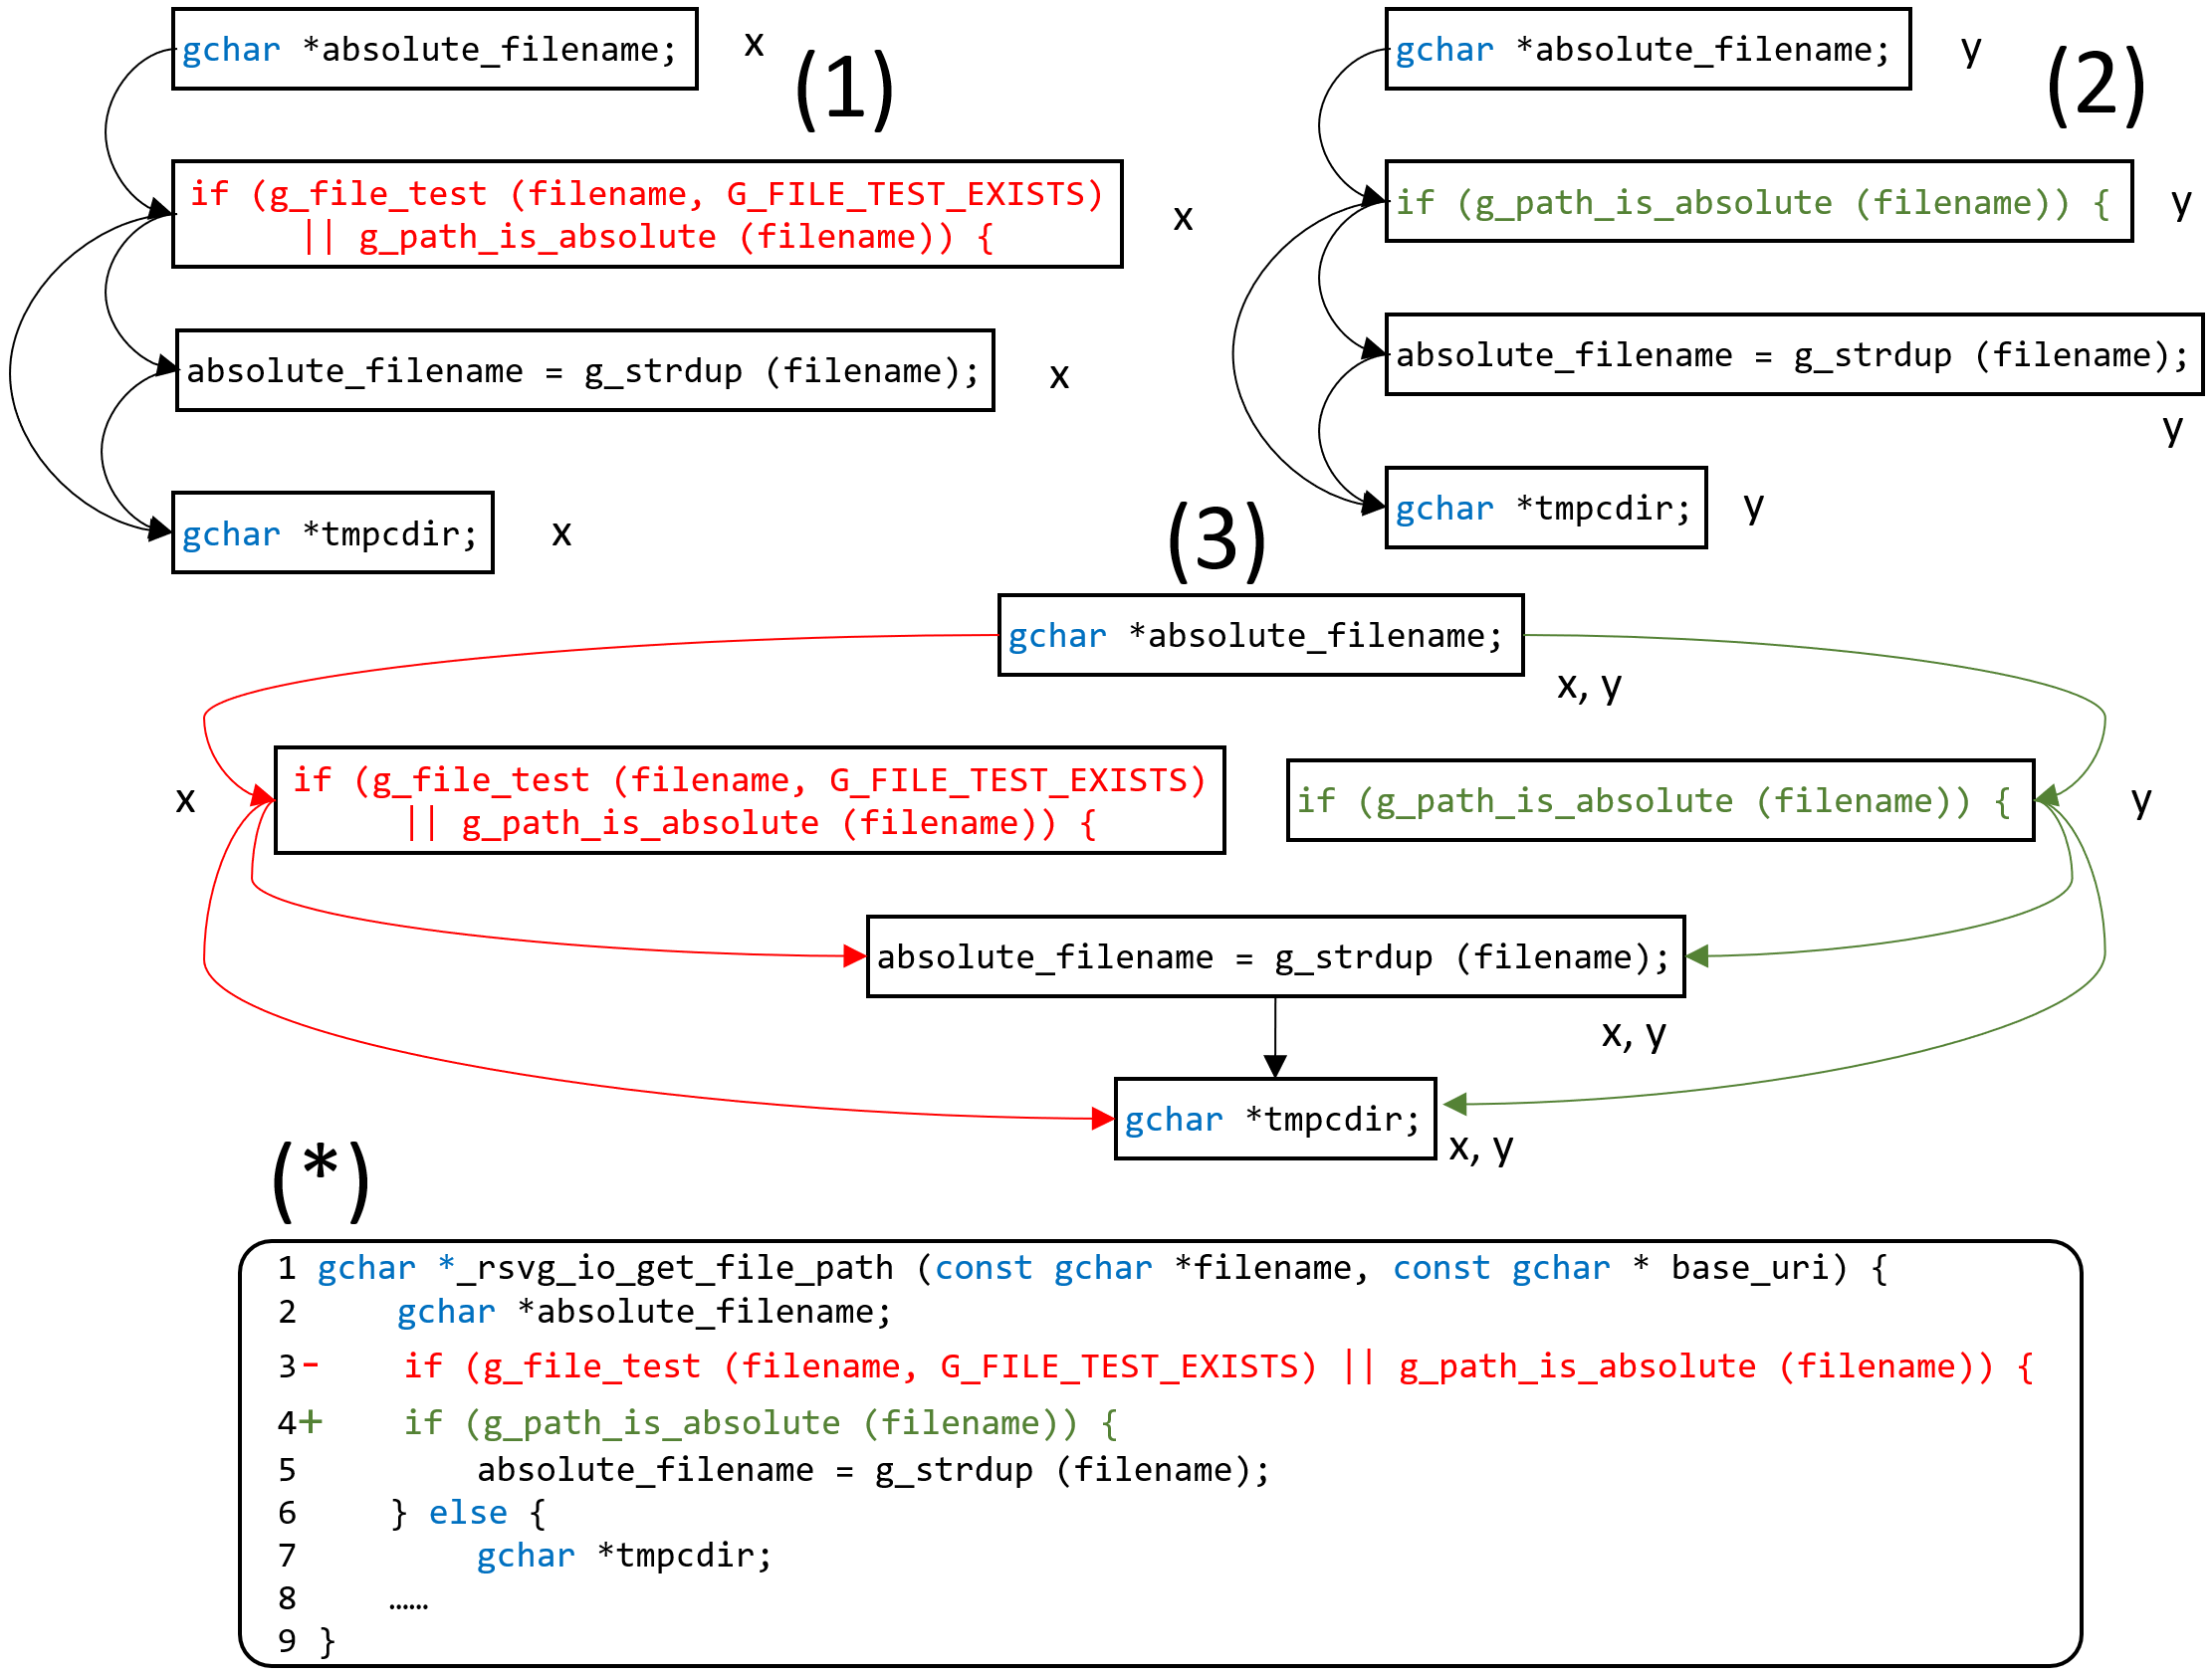
\includegraphics[width=3.4in]{multi-version-pdg.png}
	\caption{Multi-Version Program Dependence Graph}
	\label{fig:multi-version-pdg}
\end{wrapfigure}


We propose a context-aware, graph-based, representation learning model
to learn the contextualized embeddings for the code changes in a
commit that integrate both program dependencies and the contexts. To
build the contextualized embeddings, we leverage the Label,
Graph-based Convolution Network~\cite{label-gcn} to learn the
representation vector $v$ for node $n$ in the graph whose nodes
can have labels. We use labels to denote the nodes at either versions
$x$ or $y$, or at both versions $x$ and $y$.



For a changed node $n_c$, we collect all the un-changed nodes in the
context of $n_c$. The context is defined as the set of all the
un-changed nodes that are $k$-hop neighbors of $n_c$. In the
{\mvpdgxy} in Fig.~\ref{fig:multi-version-pdg}, for the changed
statement at line 4, if $k=1$, the context of that change includes the
statements at lines 2, 5, and 7 (i.e., 1-hop neighbors from line 4).




From the context nodes, we compute the vector representing the context
for a changed node $n_c$ and use it as a weight to represent the
impact of context to build the contextualized embedding for $n_c$.
From those embeddings, we compute the vector for the entire
commit and feed it to
%a SoftMax layer acting as
a classifier to~per\-form assessment classification for each CVSS
assessment type.

%Tien rewrote this para as above
%We collect the vectors of the context nodes into a matrix and use a
%fully connected layer to convert the matrix into a vector $v_{ctx}$ to
%encode the contextual information for the changed node $n_c$. The
%context vector $v_{ctx}$ is used as a weight to represent the impact
%of context on learning to build the contextualized embedding for the
%changed node $n_c$. We next concatenate all the vectors for the all
%the changed nodes $n_c$s into a matrix and use a fully connected layer
%to build the final vector $v^{com}$ for the entire commit. Finally, we
%feed the vector $v^{com}$ to a SoftMax layer acting as a classifier to
%perform assessment classification for each CVSS assessment type.


%\subsubsection{{\bf Step 2. Multi-task Learning-based Vulnerability Assessment Classification}}

%After having the {\mvpdgxy}, this step is mainly used to do the classification for seven different vulnerability assessment types. To achieve that, \tool setups seven separate but similar tasks on seven vulnerability assessment classification problems. Here, we pick one task to explain it in detail.

%The first step of the vulnerability assessment classification is to learn the summarized representation vector for the code changes in the vulnerability bring commit. In this step, \tool uses the Label-GCN \cite{} that can deal with the nodes with multiple labels (suitable for $x$, $y$, and $x,y$ labels in {\mvpdgxy})to learn the representation vector $v$ for each node $n$ in the graph. \tool then picks out all changed nodes in {\mvpdgxy} as a set. For each changed node $n^c$ in this set, \tool firstly collects the representation vector $v^{uc}$ for all unchanged nodes $n^{uc}$ within the $k$-hops in {\mvpdgxy} as the context of the changed node $n^c$. For example, in the {\mvpdgxy} in Figure \ref{fig:multi-version-pdg}, if we regard the statement in $line-4$ is the changed statement that we are focusing on. When $k=1$, the context of it includes the statements in $line-2$, $line-5$, and $line-7$. By concatenating $v^{uc}$ in a new dimension as a matrix, \tool uses a fully connected layer to summarize the matrix into one vector $v^{ctx}$ to represent the context information for the changed node $n^c$. Then, \tool uses the cross product to combine the node representation vector $v^c$ with the context representation vector $v^{ctx}$ to get the final representation vector $v'^c$ for the changed node $n^c$.


%Because the vulnerability assessment we want to get is for the whole vulnerability bring in commits, \tool concatenates $v'^c$ as a matrix and uses a fully connected layer to summarize the final code change representation vector $v^{commit}$. After having the final code change representation vector $v^{commit}$, \tool uses the SoftMax layer as a classifier to do the vulnerability assessment classification based on the $v^{commit}$.

\vspace{2pt}
\subsubsection*{{\bf Step 3. Multi-Task Learning for Assessment Classification}}

\begin{wrapfigure}{l}{0.55\textwidth}
	\centering
	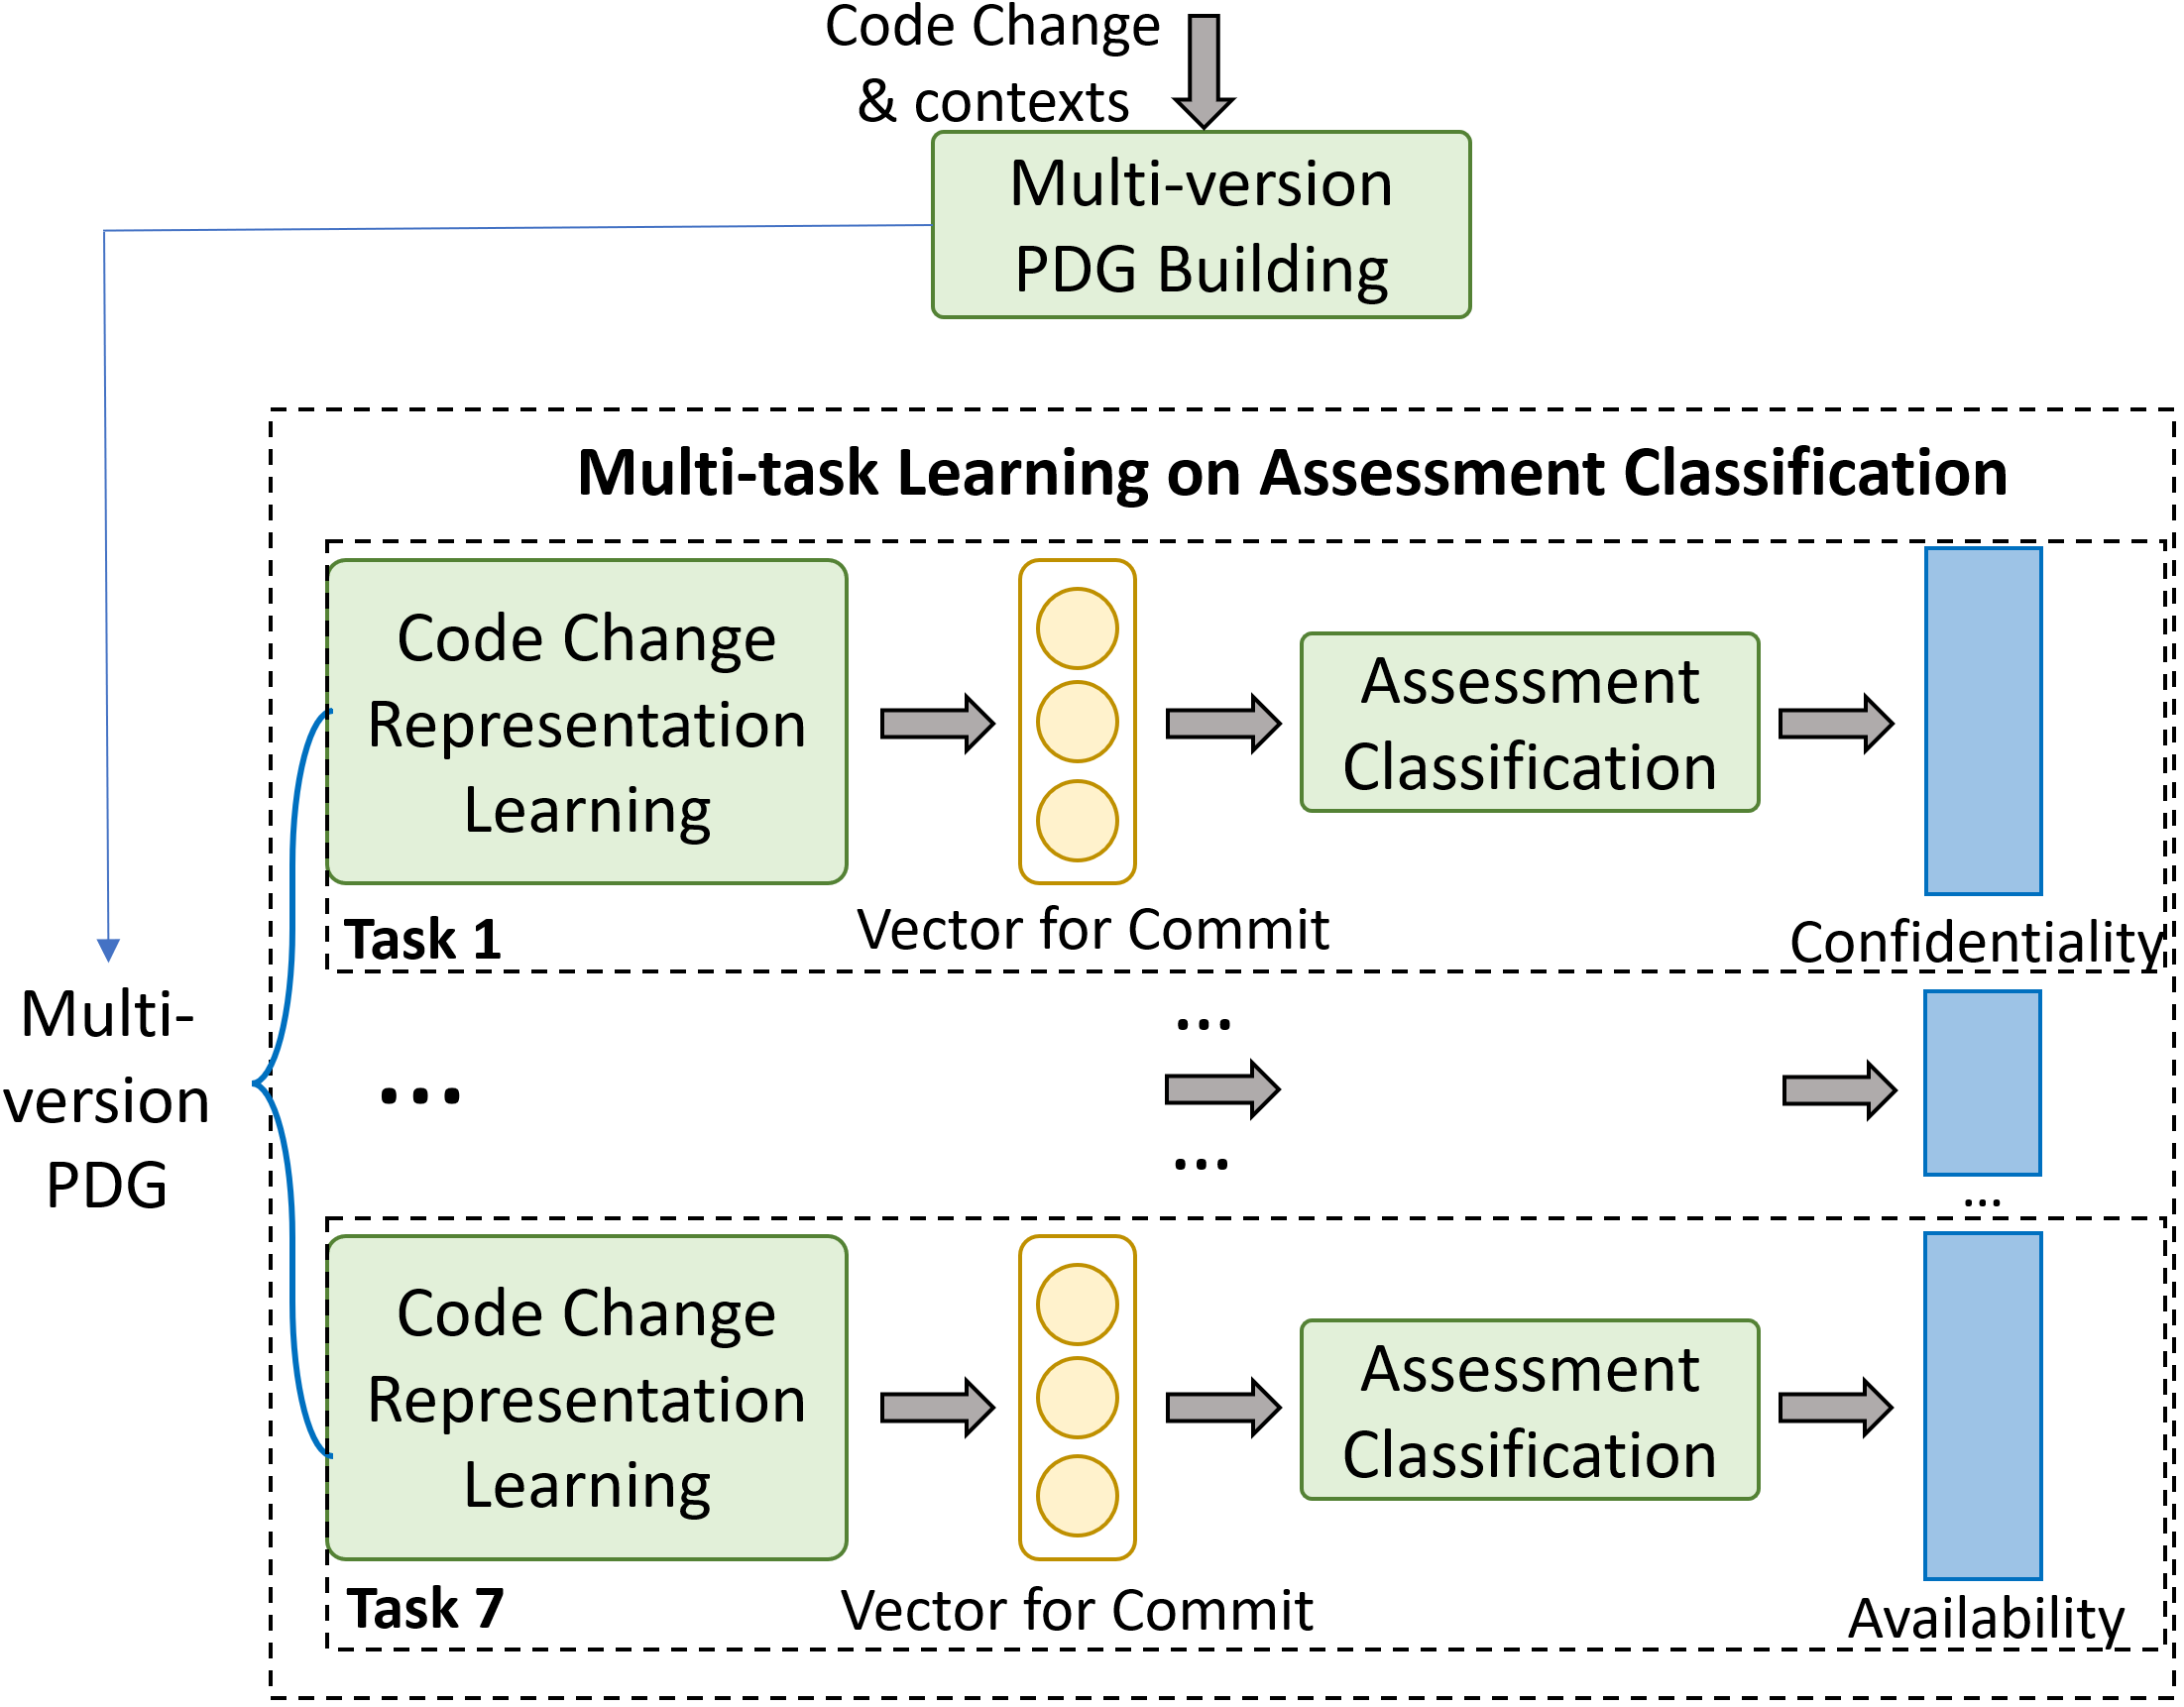
\includegraphics[width=3.4in]{overview-cat.png}
%	\vspace{-6pt}
	\caption{Automated Vulnerability Assessment}
	\label{cat-overview}
\end{wrapfigure}

%\begin{wrapfigure}{l}{0.5\textwidth}
%	\centering
%	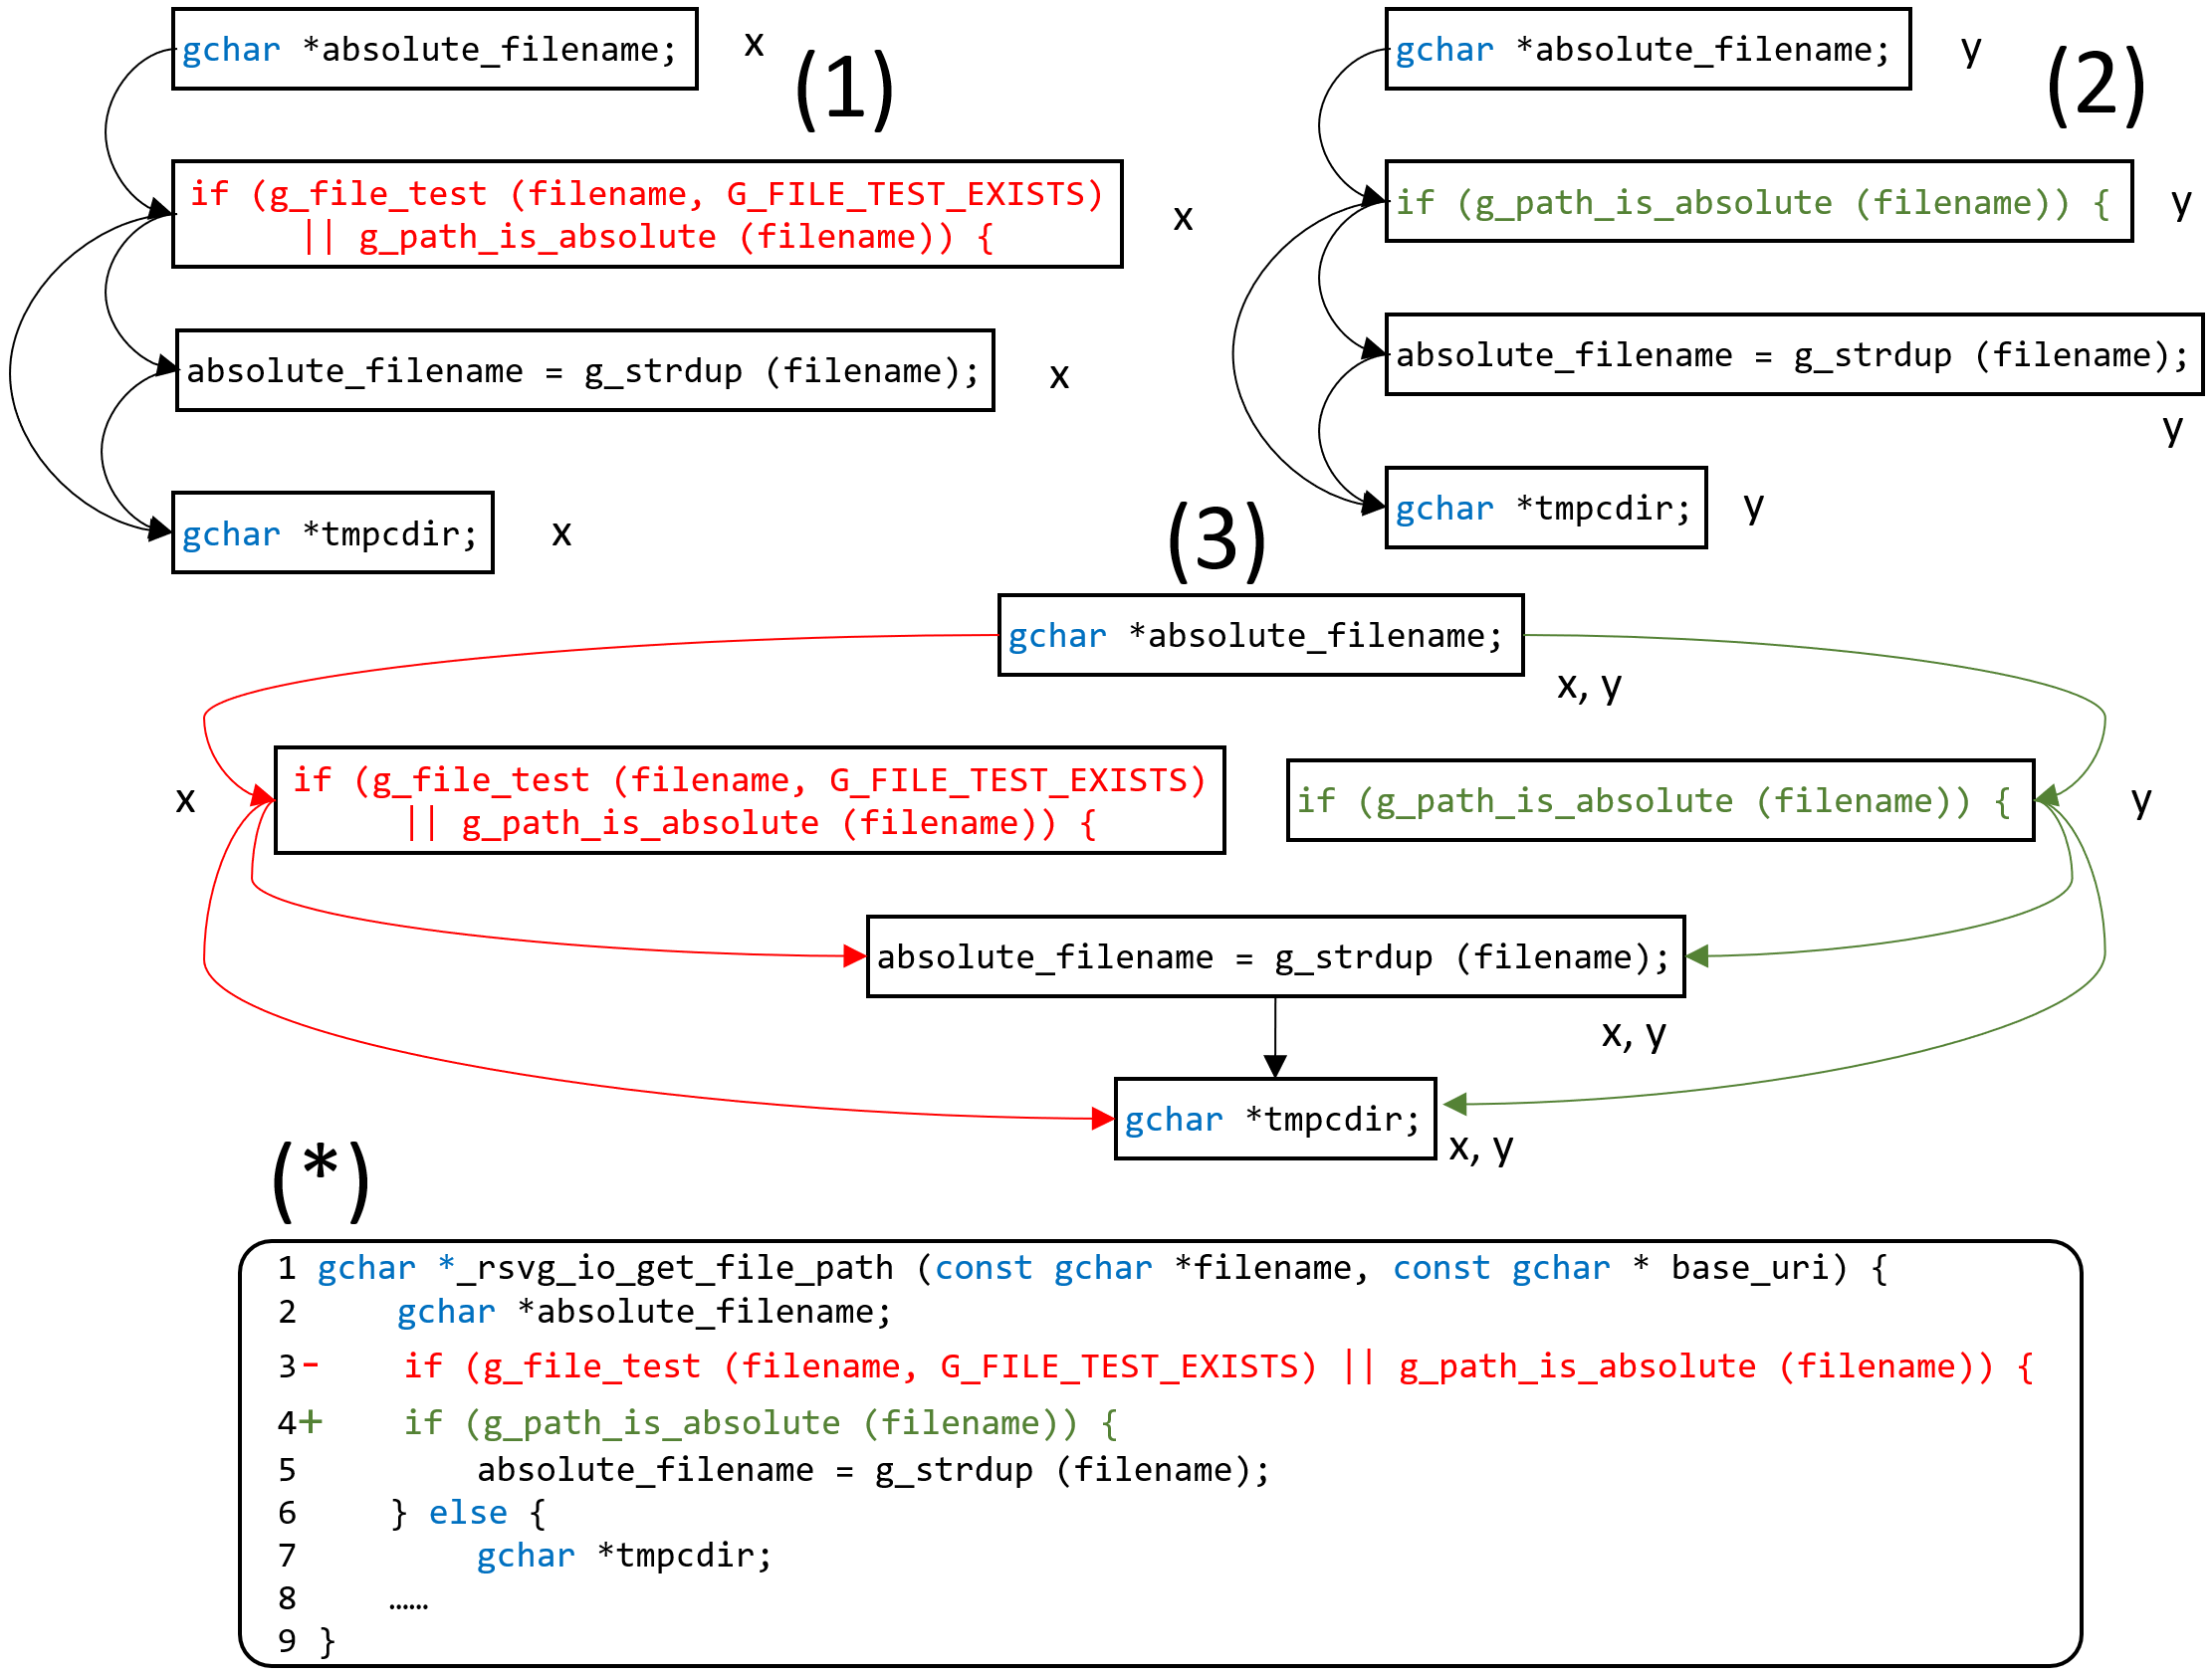
\includegraphics[width=3.4in]{multi-version-pdg.png}
%	\caption{Multi-Version Program Dependence Graph}
%	\label{fig:multi-version-pdg}
%\end{wrapfigure}

For each vulnerability assessment types (VAT), we~have a
SoftMax layer working as an assessment classification model on the
embedding of the entire commit.
%
%the SoftMax layer acts as the classifier, which takes
%the~contextualized embedding for the entire commit built on the
%{\mvpdgxy} and performs classifications.
%
To propagate the impact of the classification for one
assessment type on one another, we leverage multi-task learning among
the classification models. We use the uncertainty weighted multi-task
loss~\cite{kendall2018multi} for each classification task as the final
multi-task learning loss function and use the maximum of the average
F-score from all assessment classification tasks as the
training~target. {\bf Training and Predicting Processes}. The training/predicting processes share the above steps, except
that in training, the classification labels for the
vulnerability-introducing commits w.r.t. a VAT are known. When
predicting, {\tool} takes a vulnerability-introducing commit and code, and provides the assessment classifications for
VATs.        

{\bf Multi-Task Learning for Assessment Classification}
%\label{multi-task:sec}

In the previous sections, we have explained how {\tool} performs the
classification for a vulnerability assessment type (VAT). In this
section, we will explain our multi-task learning mechanism to perform
classifications for all seven VATs with the following prediction
classes for each VAT:

\begin{enumerate}
	\item {\bf Confidentiality}: None; Partial; Complete
	\item {\bf Integrity}: None; Partial; Complete
	\item {\bf Availability}: None; Partial; Complete
	\item {\bf Access Vector}: Local; Network
	\item {\bf Access Complexity}: Low; Medium; High
	\item {\bf Authentication}: None; Single
	\item {\bf Severity}: Low; Medium; High
\end{enumerate}

%\item {\bf Severity}: Low (0.0-3.9); Medium (4.0-6.9); High (7.0-10.0)

%With the SoftMax layer, \tool is able to do the classification for different vulnerability assessment types. In \tool, we follow the existing study DeepCVA \cite{} to do the classification on seven vulnerability assessment types. For each of them, we follows the CVSS's definition on the national vulnerability database \cite{}. These vulnerability assessment types with the classes for each type are listed as follow:

As explained, the vector $v^{com}$
representing the entire commit is passed through a SoftMax layer for
the classification for a specific VAT. Let us call it a classification
task. In CAT, the multi-task learning mechanism uses the uncertainty
weighted multi-task loss~\cite{kendall2018multi} to learn all seven
classification tasks at the same time. Specifically, for each
classification task, \tool uses a cross-entropy loss function to do
the classification as follows:
\begin{equation}\label{new-eq4}
	L = -log(Softmax(y, f(x)))
\end{equation}
Where $f(x)$ is the output of a classification task $f$; y is the
ground truth. To get the joint loss function for seven tasks with
uncertainty weighting, following Kendall {\em et
  al.}'s~\cite{kendall2018multi}, we have
\begin{equation}\label{eq5}
	L_i(W) = -log(Softmax(y_i, f^W(x_i)))
\end{equation}
\begin{equation}\label{eq6}
	L(W, \sigma_1, \sigma_2, ..., \sigma_7) = \sum_{i=1}^7\frac{1}{2\sigma_i^2}L_i(W) + log \sigma^2_i
\end{equation}
Where $W$ is the weight adding to the input, $\sigma_i$ is the
$i^{th}$ noise scalar, and $W$ and $\sigma_i$ are both trainable in
the model. With Formula (\ref{eq6}), {\tool} uses the multi-task
learning to train the seven classification models together with the
features for each task. For training, we set as the objective the
highest average F-score  for all seven
tasks. For prediction, the trained model produces the
classification results for all VATs.

%\section{Evaluation Plan}
\label{eval}

%Our {\em goals} of the evaluation plan include the studies to answer the questions:

%1) {\bf Intrinsic evaluation.} 

%2) {\bf Extrinsic evaluation.} How well do our proposed tools and methods help developers in improving the learning and usages of APIs in software libraries?

%3) How effectively do the proposed tools and methods help developers
%in real development processes?


\paragraph{\bf (1) Partial-Code Analysis Performance.} We aim
to evaluate how well {\tool} can provide the structural analysis and
semantic analysis for incomplete code fragments.  Assessing the
performance of \tool is not straightforward, mainly due to the lack of
ground-truth for partial code fragments. Thus, we could evaluate it on
programs in Java and C/C++ as follows.  First, we will train {\tool} on
complete code. For testing, we will treat each method individually and
choose a consecutive portion within the method to predict the actual
elements and dependencies, and compare them against the actual ones.
For example, in Thrust 1, if we evaluate the performance of structural
analysis infrastructure, we could compare the recovered/predicted code
structure in terms of ASTs against the actual ASTs of the original
code. For Thrust 2 in dependency analysis, we could treat each method
individually and choose a consecutive portion within the method to
predict the program dependencies, and compare them against the actual
dependencies. We will adopt the standard evaluation metrics, i.e.,
\textit{Accuracy}, \textit{Precision}, \textit{Recall}, and
\textit{F-Score}. $Accuracy = \frac{TN+TP}{TN+FP+TP+FN}$, $Recall =
\frac{TP}{TP+FN}$, $Precision = \frac{TP}{TP+FP}$, and $F{-}Score =
\frac{2*Recall*Precision}{Recall+Precision}$ where TP = True
Positives; FP = False Positives; FN = False Negatives; TN = True
Negatives.

\paragraph{\bf (2) Complete-Code Analysis Performance.}
We aim to compare the performance of {\tool} (AI/ML + PA) against the
traditional PA techniques in building structures and dependencies from
source code. We could collect a set of tools, e.g., to build the
program dependence graphs to obtain the benchmark. Then, we will
compare the results from {\tool} and other tools w.r.t. the
benchmark. We will also measure the time efficiency in building the
infrastructures such as ASTs or PDGs from all the tools under
comparison. We will use the same evaluation metrics as in the
experiments for incomplete code.

\paragraph{\bf (3) Usefulness Evaluation on Downstream Tasks.}

{\em We evaluate how well {\tool} helps in the downstream software
  engineering tasks for partial code}. For example, in bug and
vulnerability detection for code snippets, to evaluate the usefulness
of the PDGs predicted by \tool (say, PDG\textsuperscript{*}), we
will design experiments around the task of vulnerability detection at two
levels of granularity: complete code at the method-level, and partial
code at the snippet-level. For the method-level VD task, we leverage
any ML-based vulnerability detection tool, e.g.,
VulCNN~\cite{wu2022vulcnn}, an image-inspired DL-based VD model which
utilizes PDGs to predict whether a given method has vulnerabilities or
not. Here, we aim to estimate how well PDG\textsuperscript{*}s
predicted for the methods in the dataset approximate the performance
of the actual PDGs retrieved from a program-analysis tool. We could
use the same methodology for evaluating the usefulness of {\tool} in
other types of software engineering tasks.



%{\em in bug detection (BD), fault localization (FL), Regression
%  Testing in Continuous Integration (RT-CI) and automated program
%  repair (APR) approaches are in comparison with the state-of-the-art
%  approaches?}  First, we use the large-scale cross-language datasets
%with bug fixes.  To detect bugs, we will train our BD and FL
%approaches on buggy code with known buggy locations and non-buggy
%code. For APR, we train APR approaches on buggy code with its fixed
%versions to automatically learn fix patterns. Second, for evaluation,
%we follow prior research for BD, FL, and APR. \underline{In DB}, we
%will measure the precision, recall, F-measure, and the number of true
%bugs detected in Top-N (e.g., N=50). \underline{In FL}, we use the
%following: \textit{Recall at Top-N}, the number of faults with at
%least one faulty element located within the first N positions.
%\textit{Mean Average Rank (MAR)}: For precise localization of all
%faulty elements of each fault, we compute the average ranking of all
%the faulty elements for each fault.  \textit{Mean First Rank (MFR)}:
%For each project, we compute the mean of the first faulty element's
%rank for each fault.  \underline{In RT-CI}, we calculate APFD (Average
%Percentage of Faults Detected), Normalized APFD
%(NAPFD)~\cite{qu2007combinatorial} and Normalized Rank Percentile
%Average (NRPA)~\cite{bertolino2020learning}. Rank Percentile Average
%(RPA) was proposed to adapt the Average Fault Percentile to the
%prioritization problem for computing how much a predicted ranking is
%close to the actual ranking.  \underline{In APR}, we calculate the
%number of bugs automatically fixed and the ratio of correctly fixed
%bugs to the number of plausible patches when comparing with
%traditional APR approaches. Compared with DL ARP, we use: \textit{Top
%  K is the number of times that a correct patch is in the ranked list
%  of top K candidates, e.g., K=1,3,5}.

%\paragraph{{\bf (2) Comparative Study on Code Representation Learning (CLR) for BD, FL, RT-CI and APR.}}
%{\em Research question: How effective are our CRL for BD, FL, Testing and APR, and how well are they in comparison with the state-of-the-art approaches?} 
%We will perform controlled experiments to evaluate the effectiveness of our CRL in BD, FL, RT and APR, especially ablation studies on different factors in CRL. In addition, we will continue to compare our CRL with other existing CRL on other software engineering and program analysis topics. We use the same evaluation metrics as the ones in (1) for BD, FL, and APR.

%To evaluate our evaluation framework for CRL, we propose the following
%procedure. First, we will choose a well-known DL-based model for each
%application, BD, FL, RT-CI, and APR. For each of those DL-based
%models, we varied the CRL model using our design framework in Thrust
%1. We measure the quality of each CRL model and measure the
%performance of the DL-based model for each application. We will use
%statistical test to evaluate whether the high accuracy of CRL model
%leads to high performance of the same downstream model used in the
%application under study.

%\subsection{Evaluation on usefulness of the approaches in helping developers in learning API usages}

%We will perform controlled experiments to evaluate our methods and tools with developers in the loop using the actual system. We will
%gather developers and provide them various programming tasks, and
%compare the efficiency of their work with our methods/tools to the
%baseline approaches, e.g., with the Web-based code search or other
%code synthesis approaches.

%We will measure the efficiency of the work using different methods
%based on the following evaluation metrics. First, we measure
%efficiency. This could be measured by the time for developers to
%perform the tasks or the number tasks completed by developers in a
%period of time. Second, we measure coding effort: how much effort that
%developers must do to complete the API usages given the API code from
%the methods. Third, we will measure semantic correctness, either by
%the number of passing test cases or by human judgements. Finally, we
%will perform surveys on the quality of the synthesized API usage code
%to get the feedback for future improvement in the next step.

\paragraph{\bf (4) Evaluation on proposed tools and methods in helping developers in real-world development.}

We will perform a set of user studies on the usefulness of our
proposed tools in the wild by releasing our
tools in the actual real-world development. 
%We will analyze all the aspects as in the previous studies and the total uptake of the tools.  
We will record feedback to improve our tools.
%PI Wang will connect with the Industry through our \textit{The New Jersey Innovation Institute} (NJII)~\cite{njii}, an NJIT corporation focusing on helping pri%vate enterprise.
UT-Dallas has a strong tie with companies like AT\&T, Facebook, and
Bloomberg. PI Nguyen will work with his existing collaborators in
Microsoft, IBM, ABB research to perform user studies on the groups of
developers in certain tasks to evaluate the usefulness of our proposed
tools.

%%\section{Education and Dissemination Plan - Curriculum Development Activities}
\section{Dissemination and Educational Plan}
\label{edu}

\paragraph{Engaging Students into Research}

This project will create opportunities for students at UT-Dallas to
participate into cutting-edge research: PI Nguyen has currently supported
four female students (2 PhD students and 2 undergraduates), with a total
of four PhD students, two M.Sc. students, and four undergraduates.

%has worked with 6 undergraduate students (i.e., two are female
%students) and two master students (i.e., independent
%study). Additionally, PI Wang is actively doing research with a group
%of two undergraduate students (Vrushali Koli (female) from NJIT and
%Delmond Wyllis from Rowan Univ. in NJ) and \underline{six high-school
%students} in the NJ Governor's STEM Scholars Program.  PI Wang
%supervise 4 Ph.D students (one female) and 1 master student.


%(2) {\em UTD's Collegium Honors Program}:
%{\em ISU's Freshman Honor program}: 
%PI Nguyen has been engaging two freshman honor students into his
%research program since he joined UTD in 2016. 
%REU supplements will be requested to support this undergraduate research; 
%
%(3) {\em HackersUTD}: This Fall, UT Dallas Computer Science department
%welcomed 2,876 students, including 466 CS/software engineering
%freshmen, with activities and events as a way to welcome and
%familiarize students with the UT Dallas CS. We will engage members of
%this organization; 
%(3) UT Dallas works with North Texas high school
%seniors to host IT empowerment for their camps. To generate interests
%in computing studies from {\em high-school} students in Dallas area,
%we will involve them in design projects that target the use of
%software in teaching {\em K-12} subjects; 
%(2) {\em UTD's Women Who
%Compute}: The PI Nguyen has actively used this program to generate interests
%in SE research from women students. From the past, PI Nguyen has
%mentored 3 women students; 
%(Dong Fei, Kristina Gervais, Taylor Schreck); 
%(3) {\em Involving Under-represented Minorities}: We
%will attract minority students funded by GEM fellowships, involve
%high-school teachers via Alliances for Graduate Education and the
%Professoriate.
%and UT Dallas Programs for Minors: we will work
%with this program to recruit more student in minority.

%This project will also create opportunities for students at UT-Dallas:
PI Nguyen has extensive experience in engaging students in
outreach programs: (1) {\em UTD's Collegium Honors Program}: He
has been engaging several freshman honor students into his research
program since 2005. (2) {\em HackersUTD}: In Fall'19, UT Dallas CS
welcomed 2,876 students, including 466 freshmen, with activities and
events as a way to familiarize students with CS/SE. We will use the
results of this project in this program.
%
(3) UT Dallas works with {\em North Texas high school seniors to host
IT empowerment} for their camps. To generate interests in computing
studies from {\em high-school} students in Dallas area, PI Nguyen has
been involving them in design projects that target the use of software
in teaching {\em K-12} subjects; (4) {\em UTD's Women Who Compute}: he
has actively used this program to generate interests in SE research
from women students. PI Nguyen has mentored several {\em female
undergraduate students} (Weining Gao, Kristina Gervais, Taylor
Schreck, etc.); (4) {\em Involving Under-represented Minorities}: We
will attract minority students funded by GEM fellowships, involve
high-school teachers via Alliances for Graduate Education and the
Professoriate; and (5) {\em UT Dallas Programs for Minors}: we will
work with this program to recruit more student in minority.


\paragraph{Dissemination of Research and Teaching Materials}

Beside publications at professional \emph{conferences, journals} and
public Web sites, we will use the available resources at UT-Dallas
through various forums for dissemination.
%
%PI Wang is a member of DIMACS~\cite{dimacs}, the Center for Discrete
%Mathematics and Theoretical Computer Science as an NSF-funded Science
%and Technology Center (STC) and a New Jersey Commission on Science and
%Technology Advanced Technology Center. DIMACS has over 350 members
%across the U.S. PI Wang will continue to advocate our research through
%DIMACS events, research and academic programs.  PI Wang will use
%the \textit{annual NJIT Research Showcase and President Forum} to show
%our accomplishments to all NJIT people.
PI Nguyen will continue to use the following resources: (1) TExAs
Software Engineering Research (TEASER) Doctoral Symposium: where SE
researchers from the DFW Metroplex (and beyond) meet to discuss and
work on SE topics.  The mission of TEASER is to provide a supportive
space in which PhD students can present and receive feedback on their
research work, while at the same time giving both researchers and
students a venue to get to know one another and network productively.
(2) American Society for Engineering Education: PI Nguyen, with his
prior NSF-funded TUES project, has disseminated educational results
via this channel.
%He will continue to disseminate educational outcomes via this
%educational society.
(3) Leadership through Engineering Academic Diversity (LEAD): PI
Nguyen have served as mentors for this program which aims to enrich
educational experience of {\em minority engineering students}.

\paragraph{Research Community Building.}

PI Nguyen has successfully organized the 1st {\bf International
Workshop on Representation Learning for Software Engineering and
Programming Languages (RL+SE\&PL 2020)}~\cite{rlsepl}, associated with
ESEC/FSE'20. The workshop had 104 paid registers and featured one
keynote speaker (Dr. Miltos Allamanis, well-known CRL scientist at
Microsoft Research) and six technical presentations. RL+SE\&PL'20 has
sparked constructive and inspiring discussions. With its success, we
are building a diverse and active community. We plan to build on the
success of the first edition to continue this series to disseminate
ideas to a wider community, and to build a larger community bridging
SE and ML.


\noindent {\bf Undergraduate and Graduate Software Engineering (SE) Education.} 
%PI Wang teaches fundamental and core SE courses NJIT: Building Web Applications (IS218) and System Design (IS390).
PI Nguyen is one of the key SE faculty members in SE at UT Dallas. 
%
He is one of the faculty who has initiated the
Undergraduate SE Program when he was at Iowa State University.
%He has
%successfully introduced several courses including Software
%Architecture and Design (CprE339) and Software Project Management
%(CprE329). 
Taking advantage of this project, PI Nguyen will introduce a deep
learning component and a new course in NLP+SE.
%The key teaching philosophy in this course is the combination of theory and practice.
%in which students will be introduced different principles and theories in the application of NLP in SE artifacts. 
%The tentative modules include 1) basic principles, processes, and paradigms in NLP, 2) programming languages versus natural languages, 3) API usages and reuse, 4) Statisical models used in SE applications, 5) machine translation and code migration, 6) language models for source code, 7) applications of machine translation in SE, 8) word embeddings and SE applications, 9) deep learning and SE applications, etc.
%\noindent {\em Graduate SE Education} 
PI Nguyen will teach a newly developed course, 
Selected Topics on AI in SE and PL,
including relevant topics to this proposal, e.g, 
AI in bug detection, fault localization, automated repair. 
%The PI Nguyen works
%with other UTD faculty to develop a series of six to seven SE graduate
%courses that will be offered at least every semester. This year, the
PI Nguyen introduced a new graduate level course on ``AI/ML for
Code''. The PI will introduce a new graduate course on the topic of
NLP+SE.
%Tools developed by this research will be used in class projects. 
The course will focus on SE advanced methods that
aim to help advance SE with AI/ML. 
The tentative topics include 1) program analysis, 2) code
analysis with AI/ML, 3) cross-language analysis between texts and code,
4) AI/ML for code, etc.
%4) code and text retrieval in SE applications, 
%3) NLP techniques and
%type inference, 4) NLP and de-ofuscation, 5) bug-fixing and
%machine learning.




%\section{PI's Prior Relevant NSF Supports and Qualifications for this Project}
\label{prior}

%PI Wang has no prior relevant NSF supports.
%His relevant work on improving software maintenance, quality and reliability has been published in
%OOPSLA~\cite{yioopsla19}, ASE~\cite{son-2019-ase}, EMSE~\cite{noei2019towards,wang2016improving}, ICWS~\cite{venkatesh2016client}, ICSOC~\cite{wang2014developers}, and MSR~\cite{wang2013improving,wang2019extracting}.
%two ICSE submissions, and one PLDI submission.
PI Nguyen. CCF-1723215, \$260,709, 07/01/16-30/06/21, ``Collaborative
Research: Exploiting the Naturalness of Software''.
%
\noindent {\bf Intellectual Merit.} The work has the following
thrusts: (1) investigating NLP techniques for SE
applications, and (2) Developing a statistical machine translation
model for language migration.
%Investigating the integration of semantic information
%including data types, semantic roles, etc., into a language model, (2)
%Developing an accurate code-completion tool using statistical semantic
%language model, and (3) Developing a statistical machine translation
%model for language migration.
%
\noindent {\bf Broader Impact.}
%We developed practical software engineering tools, using statistical
%NL techniques for (a) code suggestion, completion, and correction
%tools, (b) assisting tools for programmers, (c) summarization, (d)
%retrieval, and (e) porting tools.
%The project has several publications at top-tier SE
%conferences, e.g., ICSE, FSE, ASE, TSE.
%including ICSE
%papers~\cite{icse05,icse07,icse09,icse10,icse11}, FSE
%papers~\cite{fse06,fse09,fse11}, ASE
%papers~\cite{ase06,ase08,ase08-2,ase09,ase10,ase11-phpsync,ase11-bugscout,ase11-idiff},
%OOPSLA papers~\cite{oopsla04,oopsla06,oopsla10}, and TSE
%papers~\cite{tse08,tse11}.
%
He has been awarded {\bf 4 ACM SIGSOFT Distinguished Paper Awards, one
  Best Paper Award, and one best ICSE Formal Research Demonstration
  Award} at the top-tier SE conferences including ICSE, FSE, and ASE,
one {\bf IEEE TCSE Distinguished Paper Award}. He has served on
Program Committees and Program Boards of ICSE, FSE, ASE, OOPSLA,
ECOOP. PI Nguyen was a Program Co-Chair of ASE'17. Since 2005, PI
Nguyen published at the top-tier Software Engineering conferences: 25
ICSE full papers, 15 ESEC/FSE full papers, 14 ASE full papers, 3
OOPSLA full papers.
%From Google Scholar, PI Nguyen's H-index
%is 49, Citations: 9,431, Citations in past 5-years: 5,879.
From CSRankings, he is ranked at the 3rd place among all US SE researchers in the past 10 years.

%making software development more accessible, enjoyable and productive;
%and therefore will broadly enhance the value that software
%professionals deliver to business and society.

%Dr. Nguyen is currently the PI of the NSF-funded project, ``
%Collaborative Research: Exploiting the Naturalness of Software'', that
%will end August 2018. The work has three thrusts of research.  (1)
%Investigating the integration of semantic information including data
%types, semantic roles, etc., into a language model, (2) Developing an
%accurate code-completion tool using statistical semantic language
%model, and (3) Developing a statistical machine translation model for
%language migration. So far, the majority of the tasks have been
%%completed except empirical evaluation in a real-word setting is
%needed.



%Several papers on our results were published through ICSE
%2010~\cite{icse10}, ASE 2010~\cite{ase10}, OOPSLA
%2010~\cite{oopsla10}, ICSM 2010~\cite{icsm10}, ICSE
%2011~\cite{icse11,nier11-1,nier11-2}, FSE 2011~\cite{fse11}, ASE
%2011~\cite{ase11-phpsync,ase11-bugscout,ase11-idiff}, and an IEEE TSE
%journal article~\cite{tse11}.

%Our next phase will be involved more with the tasks (2) and (3).

%Dr. Nguyen is currently an PI on a NSF-funded project: \#CCF-1018600,
%``Find and Fix Similar Software Bugs'', 08/15/2010 through
%07/31/2013. In this project, an empirical study will be conducted to
%collect, analyze, and understand the nature and characteristics of
%recurring and similar bugs within one and across multiple
%systems. This project is expected to advance software engineering
%knowledge on the theoretical foundation, concepts, practical
%techniques, and automated tools to (1) capture the characteristics and
%measure the similarity of code units involved in prior known fixed
%bugs, (2) identify the locations of potential buggy units and derive
%the guidelines to fix them by matching them to the relevant peer code
%units of the known bugs, and (3) support the similar bug detection and
%fixing process. Teaching modules and validation efforts in this
%project will involve students and professionals, promoting teaching
%and training software quality assurance.

%Dr. Nguyen is an expert in software building, software configuration
%management (SCM), and software refactoring. His research work on SCM
%has been published at various prestigious software engineering
%journals and conferences including clone-aware configuration
%management and operation-based version control (TSE'11~\cite{tse11},
%FASE'10~\cite{fase10}, ASE'09~\cite{ase09}), software
%refactoring-aware SCM and software merging (TSE'08 \cite{tse08},
%ICSE'07~\cite{icse07}, FSE'06~\cite{fse06}, OOPSLA'06
%demo~\cite{oopsla06}), object-oriented configuration management
%(ICSE'07~\cite{icse07}, WWW'06~\cite{www06}, ICSE'05~\cite{icse05},
%ICSM'05~\cite{icsm05}).

%His other software maintenance works include clone-related bug
%detection (TSE'11 \cite{tse11}), bug localization
%(ASE'11~\cite{ase11-phpsync}), bug localization from bug reports
%(ASE'11~\cite{ase11-bugscout}), recurring bug detection
%(ICSE'10~\cite{icse10}), API misuse detection
%(OOPSLA'10~\cite{oopsla10}, FSE'09~\cite{fse09}), recurring
%vulnerabilities detection (ASE'10~\cite{ase10}), etc.




%Since 2005, his work has been resulting several publications at
%top-tier SE conferences including 5 ICSE
%papers~\cite{icse05,icse07,icse09,icse10,icse11}, 3 FSE
%papers~\cite{fse06,fse09,fse11}, 8 ASE
%papers~\cite{ase06,ase08,ase08-2,ase09,ase10,ase11-phpsync,ase11-bugscout,ase11-idiff},
%2 WWW papers~\cite{www04,www06}, 3 OOPSLA
%papers~\cite{oopsla04,oopsla06,oopsla10}, and 2 FASE
%papers~\cite{fase09,fase10}, 2 TSE papers~\cite{tse08,tse11}.


\newpage
\setcounter{page}{1}
\pagenumbering{roman}

\bibliographystyle{IEEEtran}
%\nobibliography{oopsla19,icse20,FL,ref,autofixTools}
\bibliography{cat-refs,oopsla19,icse20,FL,ref,autofixTools,testPri,embeddingEva,reference,icse21IntVD,icse18,nsa/FL,nsa/ref,nsa/Reference,nsa/icse21IntVD}

%\bibliography{oopsla19, icseAutoFix20,bibliography,icse18,t2api17,ccf18,refs,securesync,tc10,tien,ccf09,ase10,ccf12,anomalies,completion,groums,usagemining,pattern,urls,other}

\end{document}
